\documentclass[12pt,twocolumn,tighten]{aastex62}
%\pdfoutput=1 %for arXiv submission
\usepackage{amsmath,amstext,amssymb}
\usepackage[T1]{fontenc}
\usepackage{apjfonts}
\usepackage[figure,figure*]{hypcap}
\usepackage{graphics,graphicx}
\usepackage{hyperref}
\usepackage{comment}

\renewcommand*{\sectionautorefname}{Section} %for \autoref
\renewcommand*{\subsectionautorefname}{Section} %for \autoref

%% Reintroduced the \received and \accepted commands from AASTeX v5.2.
%% Add "Submitted to " argument.
\received{\today}
\revised{---}
\accepted{---}
\submitjournal{AAS journals.}

\shortauthors{Bouma et al.}
\shorttitle{CDIPS I: Method \& Sectors 6--8}

%%%%%%%%%%%%%%%%%%%%%%%%%%%%%%%%%%%%%%%%%%
% BEGIN CUSTOM SHORT-CUT COMMANDS

% BEGIN CLUSTER TABLE
%FIXME: write code that will write these values
\newcommand{\cgXVIIInstartot}{}
\newcommand{\cgXVIIInstarcdipsI}{}
\newcommand{\gaiaXVIIInstartot}{}
\newcommand{\gaiaXVIIInstarcdipsI}{}

\newcommand{\kXIIInstartot}{}
\newcommand{\kXIIInstarcdipsI}{}
\newcommand{\dXIVnstartot}{}
\newcommand{\dXIVnstarcdipsI}{}
\newcommand{\bellXVIInstartot}{}
\newcommand{\bellXVIInstarcdipsI}{}
\newcommand{\banyanXIIInstartot}{}
\newcommand{\banyanXIIInstarcdipsI}{}
\newcommand{\banyanXIInstartot}{}
\newcommand{\banyanXIInstarcdipsI}{}
\newcommand{\banyanXInstartot}{}
\newcommand{\banyanXInstarcdipsI}{}
\newcommand{\krausXIVnstartot}{}
\newcommand{\krausXIVnstarcdipsI}{}
\newcommand{\ohXVIInstartot}{}
\newcommand{\ohXVIInstarcdipsI}{}
\newcommand{\rizzutoXInstartot}{}
\newcommand{\rizzutoXInstarcdipsI}{}
\newcommand{\roserXInstartot}{}
\newcommand{\roserXInstarcdipsI}{}

\newcommand{\cgXVIIInclustertot}{}
\newcommand{\cgXVIIInclustercdipsI}{}
\newcommand{\gaiaXVIIInclustertot}{}
\newcommand{\gaiaXVIIInclustercdipsI}{}

\newcommand{\kXIIInclustertot}{}
\newcommand{\kXIIInclustercdipsI}{}
\newcommand{\dXIVnclustertot}{}
\newcommand{\dXIVnclustercdipsI}{}
\newcommand{\bellXVIInclustertot}{}
\newcommand{\bellXVIInclustercdipsI}{}
\newcommand{\banyanXIIInclustertot}{}
\newcommand{\banyanXIIInclustercdipsI}{}
\newcommand{\banyanXIInclustertot}{}
\newcommand{\banyanXIInclustercdipsI}{}
\newcommand{\banyanXInclustertot}{}
\newcommand{\banyanXInclustercdipsI}{}
\newcommand{\krausXIVnclustertot}{}
\newcommand{\krausXIVnclustercdipsI}{}
\newcommand{\ohXVIInclustertot}{}
\newcommand{\ohXVIInclustercdipsI}{}
\newcommand{\rizzutoXInclustertot}{}
\newcommand{\rizzutoXInclustercdipsI}{}
\newcommand{\roserXInclustertot}{}
\newcommand{\roserXInclustercdipsI}{}
% END CLUSTER TABLE

% END CUSTOM SHORT-CUT COMMANDS
%%%%%%%%%%%%%%%%%%%%%%%%%%%%%%%%%%%%%%%%%%

%%%%%

%\NewPageAfterKeywords

\begin{document}

\title{
  The Cluster Difference Imaging Photometric Survey (CDIPS).
  I. Method, Light Curves, and Planet Candidates from Sectors 6--8
}

\correspondingauthor{L. G. Bouma}
\email{luke@astro.princeton.edu}

\author[0000-0002-0514-5538]{L. G. Bouma}
\affiliation{ Department of Astrophysical Sciences, Princeton
University, 4 Ivy Lane, Princeton, NJ 08540, USA}
%
\author[0000-0002-0628-0088]{W. Bhatti}
\affiliation{ Department of Astrophysical Sciences, Princeton
    University, 4 Ivy Lane, Princeton, NJ 08540, USA}
%
\author[0000-0001-8732-6166]{J. D. Hartman}
\affiliation{ Department of Astrophysical Sciences, Princeton
University, 4 Ivy Lane, Princeton, NJ 08540, USA}
%
\author[0000-0001-7204-6727]{G. \'A. Bakos}
\affiliation{ Department of Astrophysical Sciences, Princeton
University, 4 Ivy Lane, Princeton, NJ 08540, USA}
%
\author[0000-0002-4265-047X]{J. N. Winn}
\affiliation{ Department of Astrophysical Sciences, Princeton
University, 4 Ivy Lane, Princeton, NJ 08540, USA}

\begin{abstract}
  Lorem ipsum.
\end{abstract}

\keywords{
  methods: data analysis ---
  techniques: photometric ---
  %TODO: could be individual, and enumerate each cluster as well.
  (Galaxy:) open clusters and associations: general ---
  planets and satellites: detection 
}


%%%%%%%%%%%%%%%%%%%%%%%%%%%%%%%%%%%%%%%%%%
\section{Introduction}
\label{sec:intro}

The exoplanet field is evolving.
At the beginning, Doppler spectroscopy by the Geneva and California groups
led to the first exoplanet detections (CITE: Mayor 95, Butler, Marcy).
Some of these planets transited (CITE: Henry, Charbonneau).
Despite the geometric rarity of transits, photometric monitoring can
be performed in parallel; with precise spectroscopy this has not
yet been achieved.
Parallel photometric monitoring enabled thousands of planet detections
with the Kepler spacecraft (CITE: Borucki, Morton).
The abundance of planets from Kepler taught us about statistics
(CITE: Howard, Fressin, Petigura).
By nature of its design, Kepler left open two major avenues for
improvement: (i) brighter stars, (ii) rare weirdos.
TESS (CITE: Ricker), by nature of its small, wide-field cameras, and
nearly all-sky coverage, can capitalize on both.

One class of rare weirdo to which TESS is sensitive is stars in
clusters.  For brevity, we use the term ``cluster'' to refer to open
clusters, moving groups, associations, and star-forming regions.
Each of the $\sim$1000 star clusters of the Milky Way is a gift to
astrophysics, providing a sample of stars that vary widely in mass
but all have approximately the same age and composition. 

Cluster stars have been photometered from the ground for a while
(CITE: Joel thesis, Cambridge group).
A few clusters, NAME1 and NAME2, were observed by Kepler in its prime
mission (CITE: Meibom).
And a few more, most notably X,Y, and Z, were observed in K2's
ecliptic mission (CITE).

TESS holds the promise to deliver the most homogeneous and
comprehensive cluster photometric survey in history.  Based on the
cluster membership database of \citet{Kharchenko_et_al_2013} and the
TESS apparent magnitude calculator of \citet{Jaffe_Barclay_2017}, we
estimate that $10^5$ cluster members brighter than $T=16$ will be
observed in the northern ecliptic hemisphere's full-frame images.

However, there are formidable obstacles to deriving precise photometry
from the {\it TESS} images because of the relatively poor angular
resolution.  Almost all of the clusters are within 10 degrees of the
Galactic plane (see Figure~1), where the problems with crowding and
complex backgrounds are so severe that the {\it TESS}\, Science Team
has neglected that portion of the sky in their planet simulations
\citep{Sullivan_et_al_2015}. Similarly, the {\it TESS}\, Candidate
Target List deprioritizes all objects within $15^\circ$ of the
galactic plane~\citep{stassun_TIC_2018}, which includes 90\% of all
star clusters.  The large pixel size and the high stellar surface
density will make aperture photometry unreliable.  Yet, aperture
photometry is the basis of the official {\it TESS} data reduction
pipeline and almost all reduction methods that have been applied to
{\it Kepler} and {\it K2} data.


We have begun to produce photometry from the TESS images.
For the time being, we are adopting the difference imaging (or
optionally, ``image subtraction'') technique, because of its
benefits in modelling complex backgrouds in crowded regions.


In what follows, \S~\ref{sec:method} presents BLAH, and
\S~\ref{sec:results} describes BLAH BLAH.
\S~\ref{sec:discussion} discusses, and \S~\ref{sec:conclusion}
concludes.


\begin{figure*}[t]
	\begin{center}
		\leavevmode
		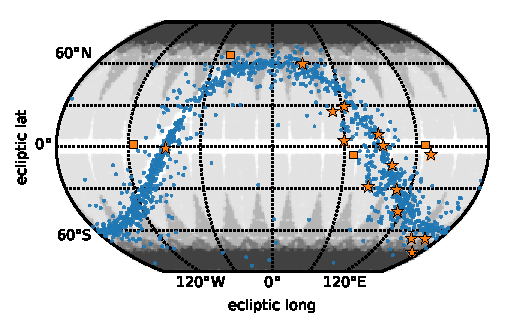
\includegraphics[width=0.7\textwidth]{cluster_positions.pdf}
	\end{center}
	\vspace{-0.5cm}
	\caption{
    {\bf TESS looks at many clusters.} Placeholder skymap.
		\label{fig:clustermap}
	}
\end{figure*}

\begin{figure}[t]
	\begin{center}
		\leavevmode
		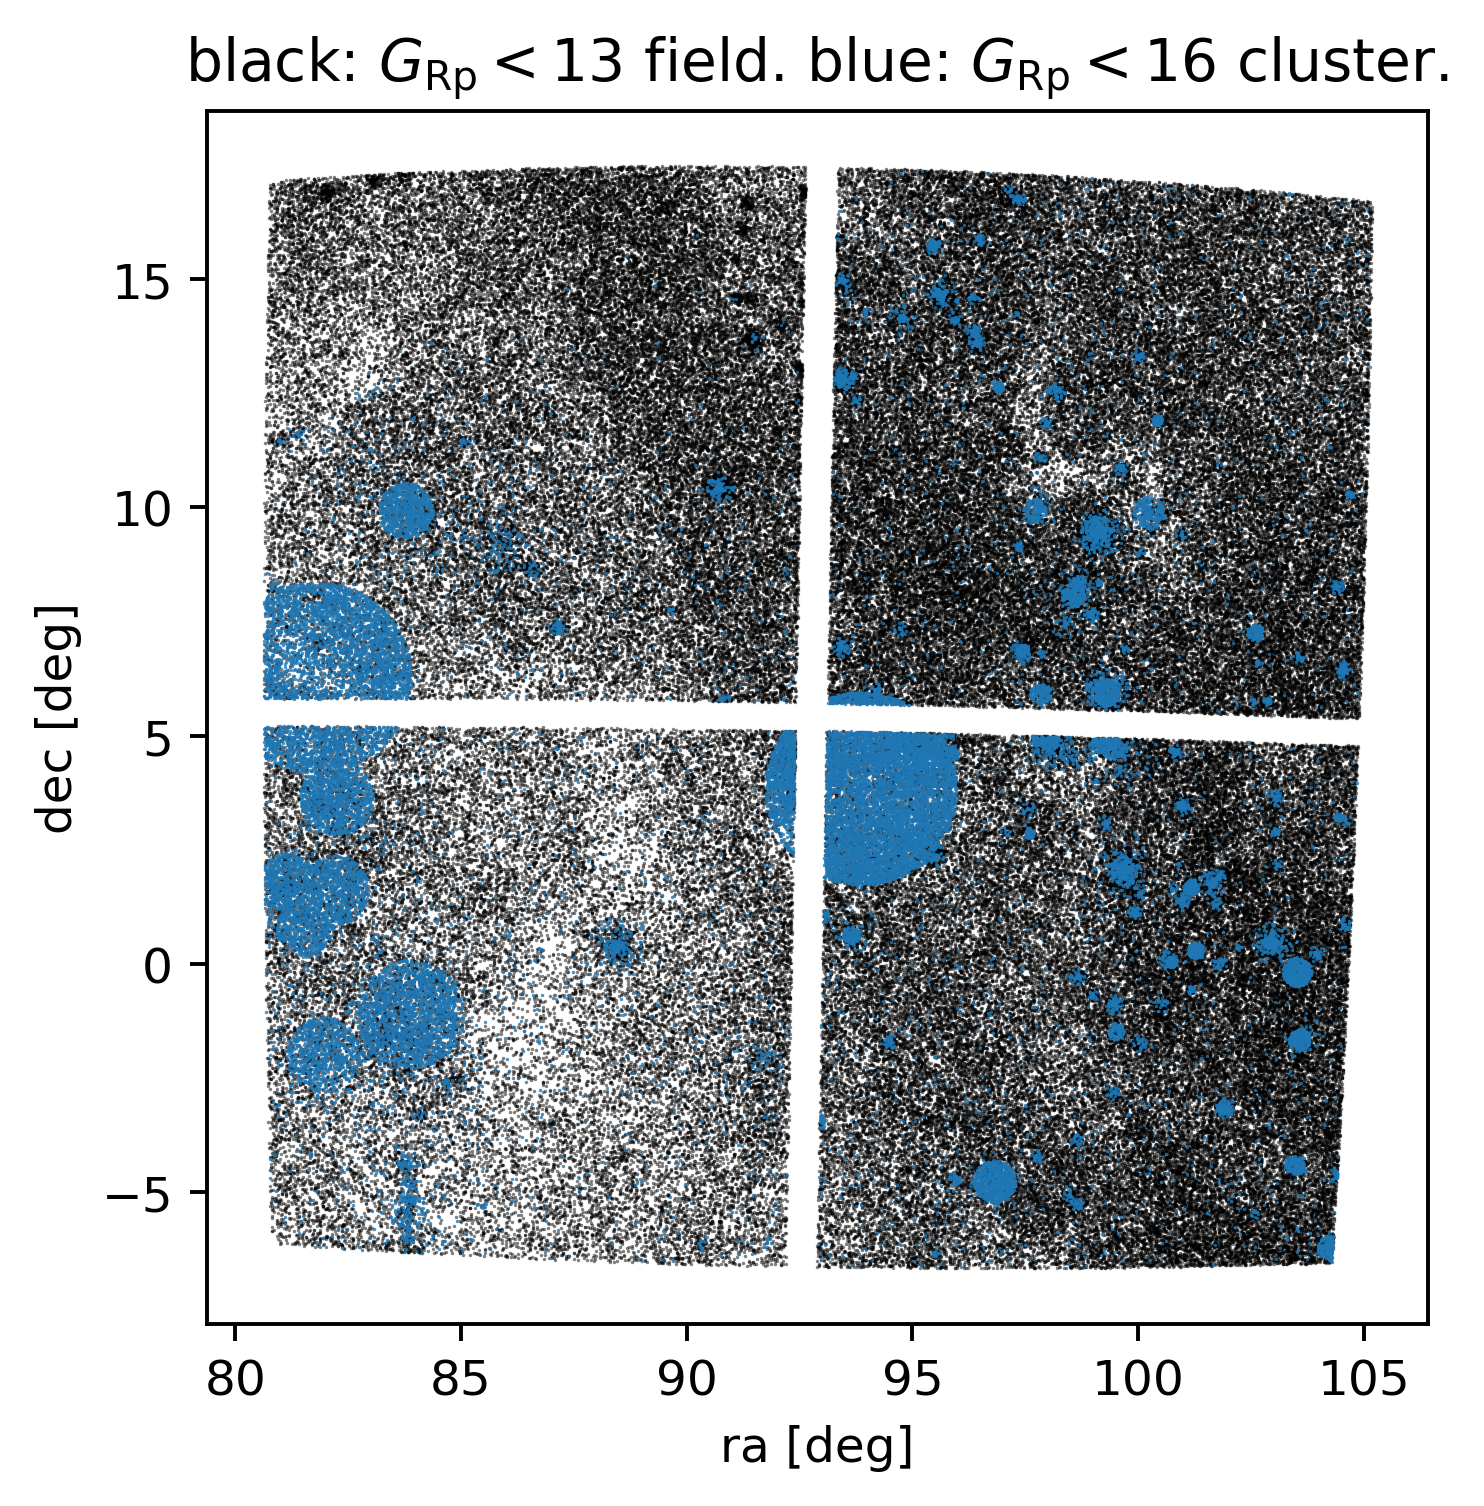
\includegraphics[width=0.49\textwidth]{cam1_cluster_field_star_positions.png}
	\end{center}
	\vspace{-0.5cm}
	\caption{
    {\bf Celestial positions of light curves from Sector 6, Camera 1.}
		\label{fig:lcradec}
	}
\end{figure}


%%%%%%%%%%%%%%%%%%%%%%%%%%%%%%%%%%%%%%%%%%
\section{Method: Star Selection}
\label{sec:starselection}

A major motivator for the CDIPS project is to increase the number of
cluster stars for which continuous photometric timeseries are
available, and thus facilitate studies of exoplanetary and stellar
processes across different times and stellar environments.
An essential aspect of the project is therefore to define a {\it
cluster star sample}, made of stars that are thought to be
members of clusters.

Performing a homogeneous membership determination for every known
cluster is beyond the scope of the current work.  Instead, we collect
various cluster membership catalogs from the literature.  We then use
them to identify cluster members within the TESS images.  In initially
selecting stars, we aim for completeness, not accuracy.  If there has
been a claim in the literature that a star should be considered a
cluster member, we would like to report a light curve for the star.
For stars that are photometrically interesting, we can perform post-hoc
cluster membership quality checks using Gaia DR2 astrometry and photometry.

Table~N describes the cluster membership catalogs we have used to
identify candidate cluster members.  Since our photometric reduction
is based on positions reported in {\it Gaia DR2}, each of our
light curve sources by default is associated with a Gaia identifier.
Correspondingly, the cluster membership determinations performed by
\citet{cantat-gaudin_gaia_2018} and \citet{gaia_hr_2018} are the
easiest case for us to merge against our light curve database.
For the TESS Sectors 1--5 light curves produced in this study, this
yielded X and Y light curves respectively.

%FIXME: make table

\subsection{Big catalogs: open clusters}
\label{subsec:oc}

\paragraph{{\it Gaia}-derived OC memberships}
At the time of writing, two relatively large, homogeneous cluster
memberships studies had been performed using {\it Gaia}-DR2: those by
\citet{cantat-gaudin_gaia_2018} and \citet{gaia_hr_2018}.

\citet{cantat-gaudin_gaia_2018} used an unsupervised membership
assignment algorithm to identify clusters in the three-dimensional
astrometric space of proper motion and parallax. They used {\it Gaia}
photometry and radial velocities to then verify the claimed
membership properties.  From their Table~2, we collect an initial 401{,}448
cluster members, in 1229 clusters, down to their limiting magnitude of
$G=18$.

\citet{gaia_hr_2018} reported memberships for stars in a smaller, more
select group of well-studied open clusters. From their Table~A1, we
collect 40{,}903 cluster members, in 41 open clusters, mostly within
$500\,{\rm pc}$. While this work also included memberships for
globular clusters, we omitted these from consideration.


\paragraph{Pre-{\it Gaia} OC memberships}
\citet{Kharchenko_et_al_2013} used proper motions calculated in PPMXL
\citep[][a combination of USNO-B1{.}0 and 2MASS
astrometry]{roeser_ppmxl_2010} and near-infrared photometry from 2MASS
\citep{skrutskie_tmass_2006} to report the existence of 2859 open
clusters and stellar associations.
We selected their ``$1\sigma$'' members according to the
combined photometric, kinematic, and spatial criteria described by
\citet{kharchenko_global_2012}.  Then, to obtain {\it Gaia}-DR2 source
identifiers for the members, we performed a crossmatch for {\it
Gaia}-DR2 sources within 5 arcseconds of the listed positions.  As an
additional constraint, we used the 2MASS photometry to predict the
$G$-band magnitudes\footnote{See
\url{https://gea.esac.esa.int/archive/documentation/GDR2/Data_processing/chap_cu5pho/sec_cu5pho_calibr/ssec_cu5pho_PhotTransf.html},
online, \texttt{2019-03-29}, or \citet{carrasco_gaia_2016}}, and
required that the measured $G$-magnitude fall within 2 magnitudes of
the predicted $G$-magnitude.  If multiple neighbors matched the
position and magnitude constraints, we took the nearest spatial
neighbor as the match.  From 373{,}226 stars, this yielded a unique
best neighbor for 352{,}332 stars (94.4\% of the sample), and a choice
between two neighbors for 17{,}774 stars. 

%FIXME is this it?
The second (non-{\it Gaia} derived) open cluster membership catalog we
used was the \citet{dias_proper_2014} catalog, which was based on
UCAC4 proper motions.
From their 1805 reported open clusters, we selected sources with
quoted membership probability above 50\%.
To obtain {\it Gaia}-DR2 source identifiers for the members, we
performed a similar crossmatch as before, looking for sources within 5
arcseconds of the listed positions, and within $\pm$2 $G$-band
magnitudes of the prediction.
From 2{,}034{,}269 stars, this yielded a unique
best neighbor for 1{,}828{,}630 stars (89.9\% of the sample), and a choice
between two neighbors for 8.7\% of the remaining sample. 

The distributions of various cross-matching statistics are shown in
Figure~\ref{fig:xmatch_info}.  The distances between matches is
typically below 1 arcsecond.  The Dias catalog shows somewhat stronger
crowding effects at the faint end compared to the Kharchenko catalog.
The Kharchenko catalog also has a more lop-sided distribution of true
{\it vs.} predicted $G$-band magnitudes.


\subsection{Smaller catalogs: moving groups and stellar associations}
\label{subsec:mg}

Stars, moving groups and stellar associations are of interest for
similar reasons as stars in open clusters.  Though fewer stars
are known to exist in moving groups, they are of particular interest
because moving groups are less crowded than open clusters, and are
often closer to the Sun.

We obtained Gaia DR2 identifiers from the results of the following
studies:
\citet{gagne_banyan_XI_2018},
\citet{gagne_banyan_XII_2018},
\citet{gagne_banyan_XIII_2018},
\citet{kraus_tucanahor_2014},
\citet{roser_deep_2011}, % OC, not MG...
\citet{bell_32ori_2017},
\citet{rizzuto_multidimensional_2011},
\citet{oh_comoving_2017}, and
\citet{zari_3d_2018}. The methods applied in these studies
vary from kinematic analyses, to astrometric analyses included
Gaia-DR1 parallaxes, to photometric searches for infrared excesses, to
spectroscopic studies including RVs, H$\alpha$
emission, and Li absorption.

For the Gagne et al{.} catalogs, we searched the Gaia-DR2 archive for
sources within 10 arcseconds of the listed positions.  If Gagne et
al{.} gave a proper motion, we required that the sign of each the Gaia
proper motion components match that of the Gagne values (the stated
proper motion uncertainties seemed to have been underestimated).  We
also imposed a $G<18$ cut on any putative matches.  Of 3012 moving
group members collected from the three combined Gagne et al{.}
catalogs, we found 2702 matches.

The \citet{kraus_tucanahor_2014}, \citet{roser_deep_2011}, and
\citet{bell_32ori_2017} studies reported members in Tucana-Horologium,
the Hyades, and 32$\,$Ori respectively.  Applying the same procedure as
for the Gagne catalogs gave 187, 684, and 119 best-neighbors
respectively, compared to 205, 724, and 141 initially reported
members.  Note that \citet{kraus_tucanahor_2014} found that only
$\sim$70\% of their listed members have spectroscopic indicators
consistent with their membership in Tucana-Horologium.

\citet{rizzuto_multidimensional_2011} also focused on a single moving
group: the Sco OB2 association. We used their reported Hipparcos
identifiers, and matched against the {\it Gaia} archive's
\texttt{hipparcos2\_best\_neighbour} table, which gave 319
nearest-neigbor stars from 436 candidate members.

Next, \citet{oh_comoving_2017} searched for comoving stars in the
$\approx$2 million stars that overlapped between Tycho-2 and {\it
Gaia}-DR1.  They found many wide binaries, and also identified a large
number of comoving groups.  We chose the 2{,}134 stars that they
reported were in groups with sizes of at least 3 stars.  Using their
{\it Gaia}-DR1 source identifiers, we matched against the {\it Gaia}
archive's \texttt{dr1\_neighbourhood} table, which gave 1{,}881
nearest-neigbor stars in groups of at least three stars
\citep{marrese_gaia_2019}.

Finally, \citet{zari_3d_2018} constructed a sample of young stars
within $500\,{\rm pc}$ using data from Gaia-DR2. Two subsamples were
made: (a) an upper main sequence (MS) sample, with 86{,}102 stars, and
(b) a pre-MS sample, with 43{,}719 stars.  Each was created from a
careful combination of distinct astrometric and photometric cuts.
These stars are the youngest, closest stars, spread across
star-forming complexes in Sco-Cen, Orion, Vela, Taurus, and other
regions of the sky.  Though many are not strictly identified with
moving groups or open clusters, their reported youth and proximity to star
forming regions justifies their inclusion in our search sample.


\subsection{Summary of selected stars}

\begin{figure}[t]
	\begin{center}
		\leavevmode
		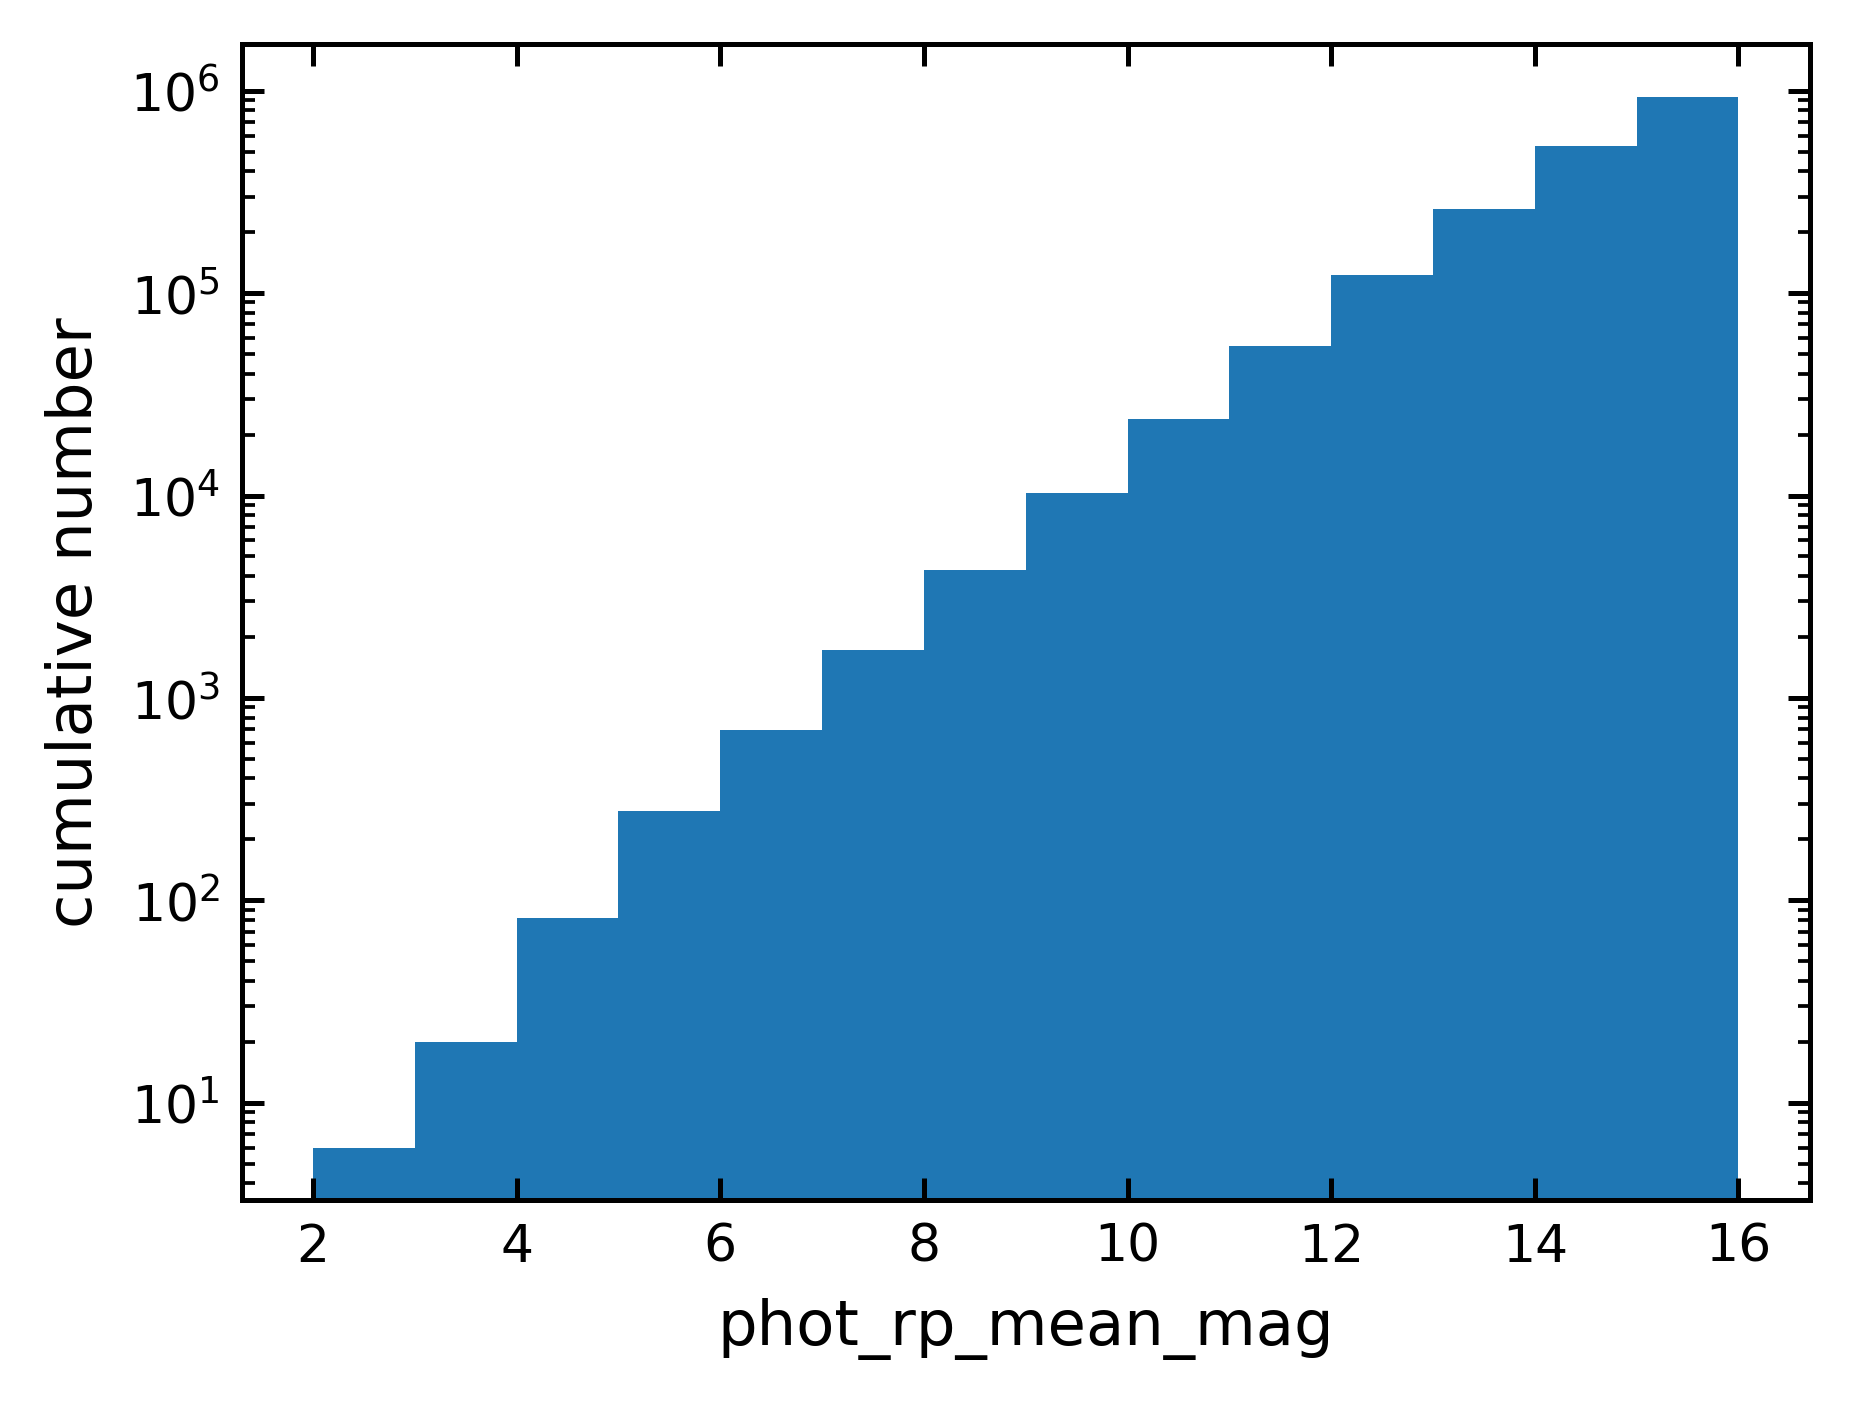
\includegraphics[width=0.45\textwidth]{star_catalog_mag_histogram_phot_rp_mean_mag.png}
	\end{center}
	\vspace{-0.2cm}
	\caption{
    {\bf Cumulative counts of candidate cluster member stars a
    function of Gaia $Rp$-band magnitude.}
	\label{fig:cdips_targets}
	}
\end{figure}

\begin{figure*}[!ht]
	\gridline{\fig{mwscmatchstats.png}{0.95\textwidth}{}}
	\vspace{-0.8cm}
	\gridline{\fig{dias14matchstats.png}{0.95\textwidth}{}}
	\caption{
		{\it Top.} Cross-match statistics from \cite{Kharchenko_et_al_2013} {\it 
			vs.} Gaia-DR2.
		{\it Bottom.} Ditto, for \cite{dias_proper_2014} {\it vs.} Gaia-DR2.
	}
	\label{fig:xmatch_info}
\end{figure*}


After collecting the aforementioned lists, we
merged them into a single table. We then queried the
\texttt{gaiadr2.gaia\_source} table to retrieve their photometric $G$,
$G_{\rm Rp}$, and $G_{\rm Bp}$ magnitudes, as well as their
astrometric measurements $(\alpha, \delta, \mu_\alpha, \mu_\delta,
\pi)$.  Finally, we required that $G_{\rm Rp} < 16$.  

All told, this procedure yielded 1{,}061{,}447 unique stars, from 13 distinct
membership catalogs.

107{,}647 of these stars, or about
10\% of the collection, have cluster memberships reported by
multiple authors.  The largest number of stars come from
\citealt{dias_proper_2014} (44.3\% of stars), \citealt{Kharchenko_et_al_2013}
(17.3\%), \citealt{cantat-gaudin_gaia_2018} (16.7\%), and \citealt{zari_3d_2018}
(11.1\%).
Stars reported in multiple catalogs have all available reference information
concatenated.  
The resulting CDIPS target star list is given in Table~N.
The distribution of target star brightnesses is shown in
Figure~\ref{fig:cdips_targets}.





%%%%%%%%%%%%%%%%%%%%%%%%%%%%%%%%%%%%%%%%%%
\section{Method: Photometry}
\label{sec:method}

\begin{figure}[t]
	\begin{center}
		\leavevmode
		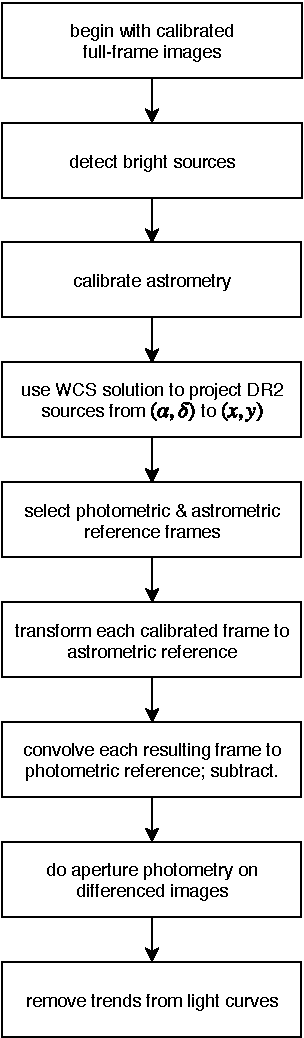
\includegraphics[width=0.3\textwidth]{pipelineoverview.pdf}
	\end{center}
	\vspace{-0.2cm}
	\caption{
    {\bf Conceptual overview of photometric reduction pipeline.}
    Details are given in \S~\ref{sec:method}.
	\label{fig:pipeline}
	}
\end{figure}

\subsection{Overview}

We reduced the TESS images to light curves by performing a sequence of
steps using stand-alone programs.
Our overall method is in the spirit of the reduction approaches described
by \citet{Pal_2009}, \citet{soares-furtado_image_2017} and
\citet{oelkers_precision_2018}; a conceptual overview is given in
Figure~\ref{fig:pipeline}.

We begin with the calibrated full frame images produced by the Science
Processing Operations Center at NASA Ames (\S~\ref{subsec:observations}).
We then perform a collection of
preparatory steps, including source extraction of bright stars,
astrometric verification, and coarse simple aperture
photometry (\S~\ref{subsec:preparation}).  Using the shape values from
the initial astrometry, we select an astrometric reference frame to
which we transform all of the calibrated images.  We construct a
photometric reference by stacking a collection of frames,
convolve the transformed frames to this photometric reference, and
subtract (\S~\ref{subsec:imagesubtraction}).  We perform aperture
photometry on the subtracted images using positions projected onto the
frame from Gaia DR2.  
We detrend the resulting light curves
(\S~\ref{subsec:lcdetrending}).  The resulting white noise and red noise properties
of the light curves, and a few
interesting cases of variability, are discussed in \S~\ref{sec:results}.




\subsection{Observations}
\label{subsec:observations}

% How did TESS observe?
% What processing steps happened in order to get the calibrated frames?
% Why did we choose to start with them?

The TESS spacecraft began science operations on July 25, 2018.  To
keep its cameras pointed opposite the Sun, the spacecraft advances by
$\approx$$28$ degrees east in ecliptic longitude every lunar month.  Data
acquired throughout each ``sector'' are downlinked at spacecraft
perigee through the Deep Space Network.  Verbose descriptions of the
spacecraft's design and operations are given by
\citet{ricker_transiting_2015} and the instrument handbook
\citep{vanderspek_2018}.

For us, the main data product of interest is the calibrated full frame
image (FFI).  Each TESS camera is read out every 2 seconds.  To produce
a manageable telemetric load, the resulting pixel values are averaged
by the onboard computer into 30 minute exposures. An on-board cosmic
ray mitigation algorithm is applied (CITE: BERTA-THOMPSON). Once
transmitted to the ground, the raw images are calibrated by the
Science Processing Operations Center.  The calibration process
includes an overscan, bias, and dark current correction, and also
divides out a flat field.  Details are discussed by
\citet{clarke_kepler_2017}, and the resulting science data products
are described by \citet{tess_data_product_description_2018}.

We begin our analysis using the calibrated images, their uncertainty
maps, and their associated headers.  The spacecraft has four cameras,
and each camera has four CCDs.  In the following analysis, all
image-level operations are thus performed on the images for each CCD,
so that at any instant of time there are 16 independent images
undergoing analysis.

While we performed numerous initial tests on the first sectors of data,
by geometric coincidence Sectors 1--5 fell away from the galactic plane.
Less than 2\% of the CDIPS target star sample
is therefore observed in the first five TESS sectors.
Though a few interesting clusters are present ({\it e.g.}, Blanco~1, NGC~2516, NGC~1901),
for the time being we opted to focus on sectors in which there were stars
of interest for our intended science.
These begin in Sector 6 (2018-12-12, spacecraft orbit \#19).


\subsection{Image Preparation, Background Removal, \& Meta-Data Collection}
\label{subsec:preparation}


\begin{figure*}[!ht]
	\gridline{\fig{astromresidual_hist.png}{0.5\textwidth}{}}
	\vspace{-0.8cm}
	\gridline{\fig{astromresidual_quiver.png}{0.5\textwidth}{}}
	\vspace{-0.8cm}
	\gridline{\fig{astromresidual_apertures.png}{0.5\textwidth}{}}
	\caption{
		{\it Top.} Histogram
		{\it Middle.} Vector
		{\it Bottom.} Apertures
	}
	\label{fig:astromresid}
\end{figure*}



Before we can perform any kind of photometry, a few janitorial tasks
are required.

First, we trim the images.  We convert the calibrated image from MAST
into a single-extension FITS image, trimmed to remove virtual rows and
columns using the \texttt{SCIROWS}, \texttt{SCIROWE}, \texttt{SCCSA},
and \texttt{SCCED} header values.

In order to pre-emptively address the background
variations present in some frames due to scattered light from the
Earth and Moon \citep[see][\S 7.3.1--7.3.4]{vanderspek_2018},
we then estimate and subtract the large-scale background.
We do this by
temporarily masking out pixels more than $2\sigma$ from the image median,
and then pass a $48\times48$ median box filter over each pixel in
the image, with reflective boundary conditions. 
We blur the resulting background estimate with a gaussian kernel,
which produces a
smooth background estimate for each image.  These steps also remove
a low-level vignetting
present in the corners of many images, which remains even after
flat-fielding \citep[see][\S 7.3.5]{vanderspek_2018}.
With the exception of scattered-light caustics, which remain in small
areas of less than 10\% of the frames, this ad-hoc procedure removes
large spatial scale scattered light patches.

% We found this background subtraction step to be particularly important
% in our subsequent difference imaging analysis. In its absense, the
% scattered light artifacts could introduce erroneous residuals into the
% kernel solution used to match reference and target images.  Including
% this step mitigated such effects, and helped produce clean
% subtractions.  Even after subtraction, a small fraction of frames also
% show sharp features (caustics) below our median box filter's size
% scale.  Such features may affect flux measurements at specific times
% in a small subset of light curves.

After subtracting the background, we mask out saturated stars using a
fixed saturation level of $8\times10^4\,{\rm ADU}$. This value was
chosen based on the onset of visible trails of bleeding charge, and is
slightly greater than the expected saturation level quoted by
\citet{vanderspek_2018}.  As described by \citet{Pal_2009}, our masks
are metadata to the image, and are only applied to the
pixel values during the specific image processing steps in which they
are necessary ({\it e.g.}, convolution). We also extend the masks
beyond purely saturated pixels to ``bloomed'' pixels horizontally and
vertically adjacent to the saturated pixels (see Figure~6 of \citealt{Pal_2009}).

Finally, for frames with the \texttt{DQUALITY} bit-flag corresponding
to the ``momentum dumps'' and ``coarse pointing modes'' described by
\citet{vanderspek_2018}, we omit the entire frame.  This removes
on average a few frames per sector. Through visual inspection, we see
that the stars on these frames are extremely smeared, and are unlikely
to produce useful science data.
In addition, we use the sector-specific data release
notes\footnote{\url{ archive.stsci.edu/tess/tess_drn.html}} to
identify further times with anomalous spacecraft performance,
which we omit from consideration.
%For Sectors 1 through 5, these
%include coarse pointing windows from orbits 10, 13, 14, and an
%instrumetal anomaly window in orbit 15.
For Sectors 6 through 8, these include three days at the beginning of
Sector 6 dedicated to acquiring pixel response function data, and also
about three days during Sector 8 lost to an instrument anomaly.
%FIXME for sectors 6 thru 8

Having prepared the images, we perform some initial analysis steps
to produce metadata
needed during image subtraction.  

First, we use \texttt{fistar} to perform source extraction on bright
stars in each image.
uring the initial source
extraction, we also fit elongated gaussians to the bright stars,
yielding the shape parameters $(s,d,k)$, where the flux as a function
of position is assumed to take the form
\begin{align}
  f_{\rm elong}(\vec{x}) &= B + A \exp \{ -0.5 \times ( 
    s(\Delta x^2 + \Delta y^2) + \\
    \nonumber
    &d(\Delta x^2 - \Delta y^2) +
    k(2\Delta x \Delta y)
  )  \},
\end{align}
for $\Delta x = x-x_0$, and $\Delta y = y - y_0$.  For a nearly
circular shape profile, the sharpness $s$ is related to the FWHM as
${\rm FWHM} \approx 2.35\sqrt{s}$ \citep[{\it e.g.},][]{Pal_2009}.
These shape parameters are later used when selecting an astrometric
reference (\S~\ref{subsec:imagesubtraction}).  We note that the fast
focal ratio of the TESS cameras introduces significant comatic
aberrations to the images: stars closer to the center of the field are
more round, while stars towards the edges are more triangular.

For the astrometric solution, we use the WCS and SIP coefficients
derived by SPOC and included in the FFI headers
\citep[][Sec.~8]{pence_fits_2010}.  We explored the possibility of
using \texttt{astrometry.net} \citep{lang_2010} to derive our own
astrometric solutions for each frame, but found that the astrometric
residual (the mean separation between projected and measured
positions) was consistently a factor of 1.5-2 times higher in our WCS
solutions than in those given by SPOC (perhaps attributable to the
algorithm used to select stars and measure their positions).

With the resulting WCS information, we then project a source catalog
onto each frame.  Initially, we planned to photometer all Gaia-DR2
sources in each field down to a cutoff of $G_{Rp} < 16$.  However, we
found that for the galactic plane fields this produces an excessively
large number of sources (millions of stars per
$12^\circ\times12^\circ$ CCD).  We therefore limited our source
catalog for each frame to be
a combination of the CDIPS target stars ($G_{Rp} < 16$), and
all Gaia-DR2 sources down to $G_{Rp} < 13$.  We use the expected
projected of these sources to center the apertures in our photometry,
rather than attempting to detect the positions.  Such
``forced-aperture photometry'' is preferable to performing source
extraction in the crowded fields that are central in this work.  The
Gaia-DR2 epoch is J2015.5, so even the fastest-moving stars with
proper motions of $\sim$$1\,{\rm arcsecond}\,{\rm yr}^{-1}$ are still
well within one pixel of their predicted positions in the TESS images.
The projection from catalog sky-coordinate positions to pixel
coordinates is performed using an analog of the \texttt{wcs-rd2xy}
program that performs the standard matrix algebra \citep{lang_2010}.
The source catalog look-up is performed using
\texttt{gaia2read}\footnote{\url{github.com/samuelyeewl/gaia2read}}
\citep{kim_2018_gaia2read}.

The astrometric residual is displayed for one photometric reference
frame (to be described shortly) in
Figure~\ref{fig:astrometricresidual}.
A few salient points can be made.
First, the typical median precision of the WCS solution is a bit below
0.1 pixels, and its $90^{\rm th}$ percentile is typically less than
0.3 pixels\footnote{In fact, in our reduction we automatically impose
that the median residual and 90th percentile remain below 0.2 and 0.4
pixels, respectively.}.
The distribution has a outlier tail of saturated stars which were
masked, and thus do not have measureable centroid positions.
The errors are typically largest in the corners of the field of view,
where the non-linearity of the focal plane is most significant, and
where the corrections required by the SIP coefficients are largest.
The final sub-panel of Figure~\ref{fig:astrometricresidual} is a
sanity check on the location of the projected positions, and also
gives some context for our chosen aperture radii of 1, 1.5, and 2.25
pixels.

Finally, we use \texttt{fiphot} to perform aperture photometry on the
bright stars from the
source list, by summing the counts inside appropriately-weighted
circular apertures centered on the projected positions from Gaia DR2. 
The pixel weights $w_{x,y}$ are equal to the fraction of the pixel
that falls within the aperture.  They are thus unity for pixels
entirely within the aperture, and fractional along the aperture
boundary (see \citealt{Pal_2009} Fig 17). 
The background levels are measured in annuli around each aperture
center.  The raw flux of the object after background removal is then
(\citealt{Pal_2009} Eq 65)
\begin{equation}
  f = \sum_{x,y} w_{x,y} (I_{x,y} - B) = f_{\rm total} - B r_0^2.
  \label{eq:simple_aperture_phot}
\end{equation}
The resulting measurements, for instance of the background level of
each aperture, and the number of ``good'' objects that are detected,
are later used to select photometric reference frames.


\subsection{Image Subtraction}
\label{subsec:imagesubtraction}

The core operation of ``classical'' image subtraction
attempts to match a photometric reference $R$ and a target image $I$ by 
computing and applying a convolution kernel.
For ground-based data, this ``match'' typically corrects for
differences in seeing or transparency between the reference and
target; for space-based data, the match might correct for spacecraft
jitter, or thermal and corresponding PSF variations.
The kernel, once applied to the high signal-to noise reference,
produces a model image, $M_{xy}$,
\begin{equation}
    M_{xy} = (R \otimes K)_{xy} + B_{xy},
\end{equation}
where $B_{xy}$ is a component of the model image that allows for
background variations.
We model the background separately, so we set $B_{xy}=0$.
The convolution kernel $K$ is typically decomposed onto a
basis, $K = \sum_i c_i K_i$, and the coefficients are found
by minimizing
\begin{equation}
    \chi^2 = \sum_{xy} \left( \frac{I_{xy} - M_{xy}}{\sigma_{xy}} \right)^2,
    \label{eq:chisq_conv}
\end{equation}
where $\sigma_{xy}$ is the uncertainty in the target image pixel values.
Photometry is then performed on the difference image $D_{xy}$, where
$D_{xy} = I_{xy} - M_{xy}$.
For this work, the uncertainty in each target image pixel is
taken to be a constant.	

The procedure described above was first proposed by \citet{Alard_Lupton_1998}.
It was reviewed and clarified by \citet{miller_optimal_2008}.
The choice of how to decompose the kernel was further clarified by
\citet{bramich_new_2008}, who showed that using a delta function
had a few select advantages compared to a basis of gaussians.
We perform the convolution using \texttt{ficonv}, and opt for
the implementation of Bramich's method (see \citealt{Pal_2009} Section 2.8).

For posterity, we note a few implementation details.
We must select two ``reference frames'' for image subtraction:
(1) the astrometric reference; (2) the photometric reference.

To choose the astrometric reference, we search for frames with
the largest and roundest stars (big $s$, small $d$ and $k$ values).
We also require
that the frame must minimal background noise, as measured in annuli
around the bright stars selected in \S~\ref{subsec:preparation}.
Finally, the astrometric reference frame must have, relative to the 
other frames being
considered, a large number of detected sources.
We sort the frames using these metrics, and then select the
astrometric reference from successive intersections of each sorted
list.
Using the algorithm presented by \citet{pal_astrometry_2006}, we then
use the \texttt{grtrans} tool to
calculate an affine transformation that maps each calibrated frame
to the astrometric reference.
We use the flux-conserving interpolation
scheme described by \citet{Pal_2009} to minimize photometric errors
incurred during this step --
standard bilinear or bicubic interpolation do not achieve flux
conservation.  
The largest component of the transformation is typically a translation,
of order 2 arcseconds, or about 0.1 TESS pixels.
%FIXME: EXPLAIN THIS BETTER

The second reference frame is the
photometric reference, which is used both to calculate the
convolution kernel, and to obtain a
reference flux for each star.  
To minimize Poisson errors, our photometric refernce is a median average of
$N=50$ selected frames.
The sub-frames are chosen to have low scatter in their photometry,
and low background measurements, using the metadata collected
in \S~\ref{subsec:preparation}.
We convolve the 50 best candidate photometric references to the best
photometric reference, and then perform a median combination of the
frames to make the photometric reference.

%\begin{enumerate}
%  \item Lowest median scatter in photometry
%  \item Lowest median error in photometry
%  \item Lowest median background measurement
%  \item Lowest median absolute deviation in background measurements
%  \item Largest number of stars detected by \texttt{fiphot} with good
%    flags.
    % fiphot files used for all of this.
%\end{enumerate}

To measure the reference flux for each star, we go a bit further.
First, we perform forced simple aperture photometry to measure
the flux for each source.
The local background is estimated in annuli, with neighboring stars
masked out during the background measurement.
If we were to stop here, {\it it would be a bad mistake}.
The reference flux for faint stars would be overestimated, due to
crowding.
The relative amplitude of photometric signals would correspondingly
be biased small, hindering exoplanet detection.
Therefore, after performing simple aperture photometry on the 
reference frame, we fit for an for aperture-size specific zero point
that relates each star's catalog $T$-band magnitude to the
measured flux.
The $T$-band magnitude is calculated according to Equation~1 of 
Stassun et al (2019, CITE).
Crowding is minimzed down to Gaia's resolution limit.
We then use the known catalog magnitude to predict the expected
photometric reference flux.

The final instrumental flux values we report (for example,
the \texttt{IFL1} column) are similar to \citealt{Pal_2009} Equation~83:
\begin{align}
f &= f_{\rm subtracted} + f_{\rm reference} \\
&=
\frac{1}{|| K ||_1^2} \sum_{x,y} S_{x,y} (w \otimes K)_{x,y}
+
g \left(T_{\rm cat} \right),
\label{eq:ism_flux_measurement}
\end{align}
for the subtracted image $S$, which is equal to $I -  R\otimes K$,
where $I$ is the original image transformed to the astrometric
reference, $R$ is the photometric reference, and $K$ is the convolution
kernel.
The weights $w$ from the circular aperture mask are matched to
the image convolution.
The function $g$ takes as input the target star's
catalog magnitude $T_{\rm cat}$, and returns the reference flux.
Its coefficients have been fit per the procedure 
discussed in the preceding paragraph.
%FIXME: derive this equation. why exactly does this work?

A few brief notes on the algorithm to actually solve for the 
coefficients to the convolution kernel.
The procedure implemented in \texttt{ficonv} is to grid up
the image, and within each grid element find the brightest non-saturated
star. These isolated ``stamp'' stars are then used to solve for the
coefficients of the kernel, by minimizing
Equation~\ref{eq:chisq_conv}.

%NOTE : this is kind of incomprehensible
%CHECK: does the polynomial weighting actually do what you want it to do?
For the choice of basis, we opt for a delta-function kernel with an additive
flux scaling term (\citealt{soares-furtado_image_2017} Section 3.3.1
gives the equations).
The spatial variations of the PSF are captured by weighting the 
delta function and the flux scaling terms with varying
polynomial orders across the image.
Choosing this kernel introduces three additional
free parameters:
(1) the kernel box-size;
(2) the maximum order of the polynomial weighting the delta function terms;
(3) the maximum order of the polynomial weighting the flux scaling.
We performed a grid-search to tune these parameters, in
which our main metrics for success included the measured RMS as
a function of magnitude, and also the recovered SNR of transits from
known TOIs (CITE: Guerrero et al in prep 2019).

Varying the kernel box-size, we found that kernels with box-length smaller than the 
typical TESS FWHM at field center ($\approx$3 pixels) produced light curves
with the highest average scatter.
Increasing the kernel box-size from a $3\times3$ box to a $7\times7$ box led
to about a 50\% reduction in RMS for bright stars, and no difference for 
faint stars.
The largest kernels, of $(11\times11)$ pixels, had on average slightly lower 
signal-to-noise for recovered transits than for kernels of intermediate size.
We settled on a kernel box-size of $(7\times7)$ pixels, in part because the 
FWHM at the camera corners can grow by factors of $\approx$2 relative to the 
field center.

Varying the polynomial orders, we found that the highest order polynomials 
retrieved transits with $\approx10\%$ worse SNR compared to lower order
polynomials.
Varying the polynomial orders between 1 and 4 did not produce large 
differences.

Averaging over all TOIs present in the camera we used for these experiments, 
we found that different choices 
of kernel parameters produced variations of $\lesssim 12\%$ in the retrieved 
transit SNR.  
For computational expediency, we therefore chose a $(7\times 7)$ kernel with 
second-order spatial polynomial weights in the basis functions.
However, we caution that within our parameter-tuning experiments, the 
recovered SNR of perhaps a third of the TOIs varied by up to a factor of two,
which in a few 
cases would have lead to non-detections of objects near the noise floor.
In the longer term, developing an image-subtraction method that marginalizes 
over uncertainties of how to chose ``optimal'' kernels would be desirable.
Pixel-level image subtraction methods that omit these 
parameters entirely 
are also worth exploring \citep{wang_pixel-level_2017}.

With a kernel selected, and the convolution and subtraction performed, 
we calculate the instrumental fluxes on each frame per 
Equation~\ref{eq:ism_flux_measurement}. 
We do this with three different aperture sizes: for this work, circles
of radii 1 pixel, 1.5 pixels, and 2.25 pixels.
These sizes were chosen to roughly span the range of optimal aperture
sizes for stars in our sample, as calcuated in the pre-flight
\citet{Sullivan_et_al_2015} work.
To finally convert from a list of 
sources on each frame to a list of flux values at any given time, we use the 
\texttt{grcollect} transposition tool.

\subsection{Light Curve Detrending}
\label{subsec:lcdetrending}

The preceding steps produce light curves that include both instrumental
systematics as well as astrophysical variability.  The detrending
approach adopted by the HAT group typically proceeds in a few
sequential stages (see discussions from {\it e.g.}
\citealt{bakos_2010,huang_high-precision_2015,zhang_precision_2016}).
Given the heritage of our pipeline, we briefly discuss these, and then
explain why we omit most of the steps described.

The first detrending step commonly performed on ground-based data is
``magnitude-fitting'': the raw magnitudes measured from the difference
images are fit by a polynomial that depends on a combination of CCD
position, sub-pixel position, and optionally catalog magnitude and
color \citep[][Sec.~5.5]{zhang_precision_2016}.

The second step is to decorrelate against external parameters that are
known to affect the stellar flux measurements (EPD,
\citealt[][~Appendix]{bakos_2010}).  For ground-based data this may include zenith
angle, or changing PSF parameters.  For TESS data, this might include
CCD temperature, or perhaps some measure of the scatter in the spacecraft
pointing (CITE: Vanderburg 2019).

The final step is to then decorrelate the measured brightnesses of
stars against each other (TFA, \citealt{kovacs_trend_2005}).  
This accounts for variations due to unknown systematic
instrument changes that affect many stars.


%FIXME TURGID PROSE
In \S~\ref{sec:flux_vs_external_parameters}, we show that the
``external parameter'' dependence visible in the TESS data is rather
complex: ordinary linear model-fitting, as well as an initial attempts
at non-linear model fitting, are poor descriptions of the data.  
In a similar vein ``magnitude-fitting'' is minimally justified, given
how the TESS magnitudes correlate against these external parameters.
We go on to show (\S~\ref{sec:tfa_is_good_enough}) that a plausible
detrending approach for the purpose of transit discovery is to simply
decorrelate against other nearby stars with standard TFA.


\subsubsection{Flux versus external parameters}
\label{sec:flux_vs_external_parameters}

\begin{figure*}[t]
	\begin{center}
		\leavevmode
		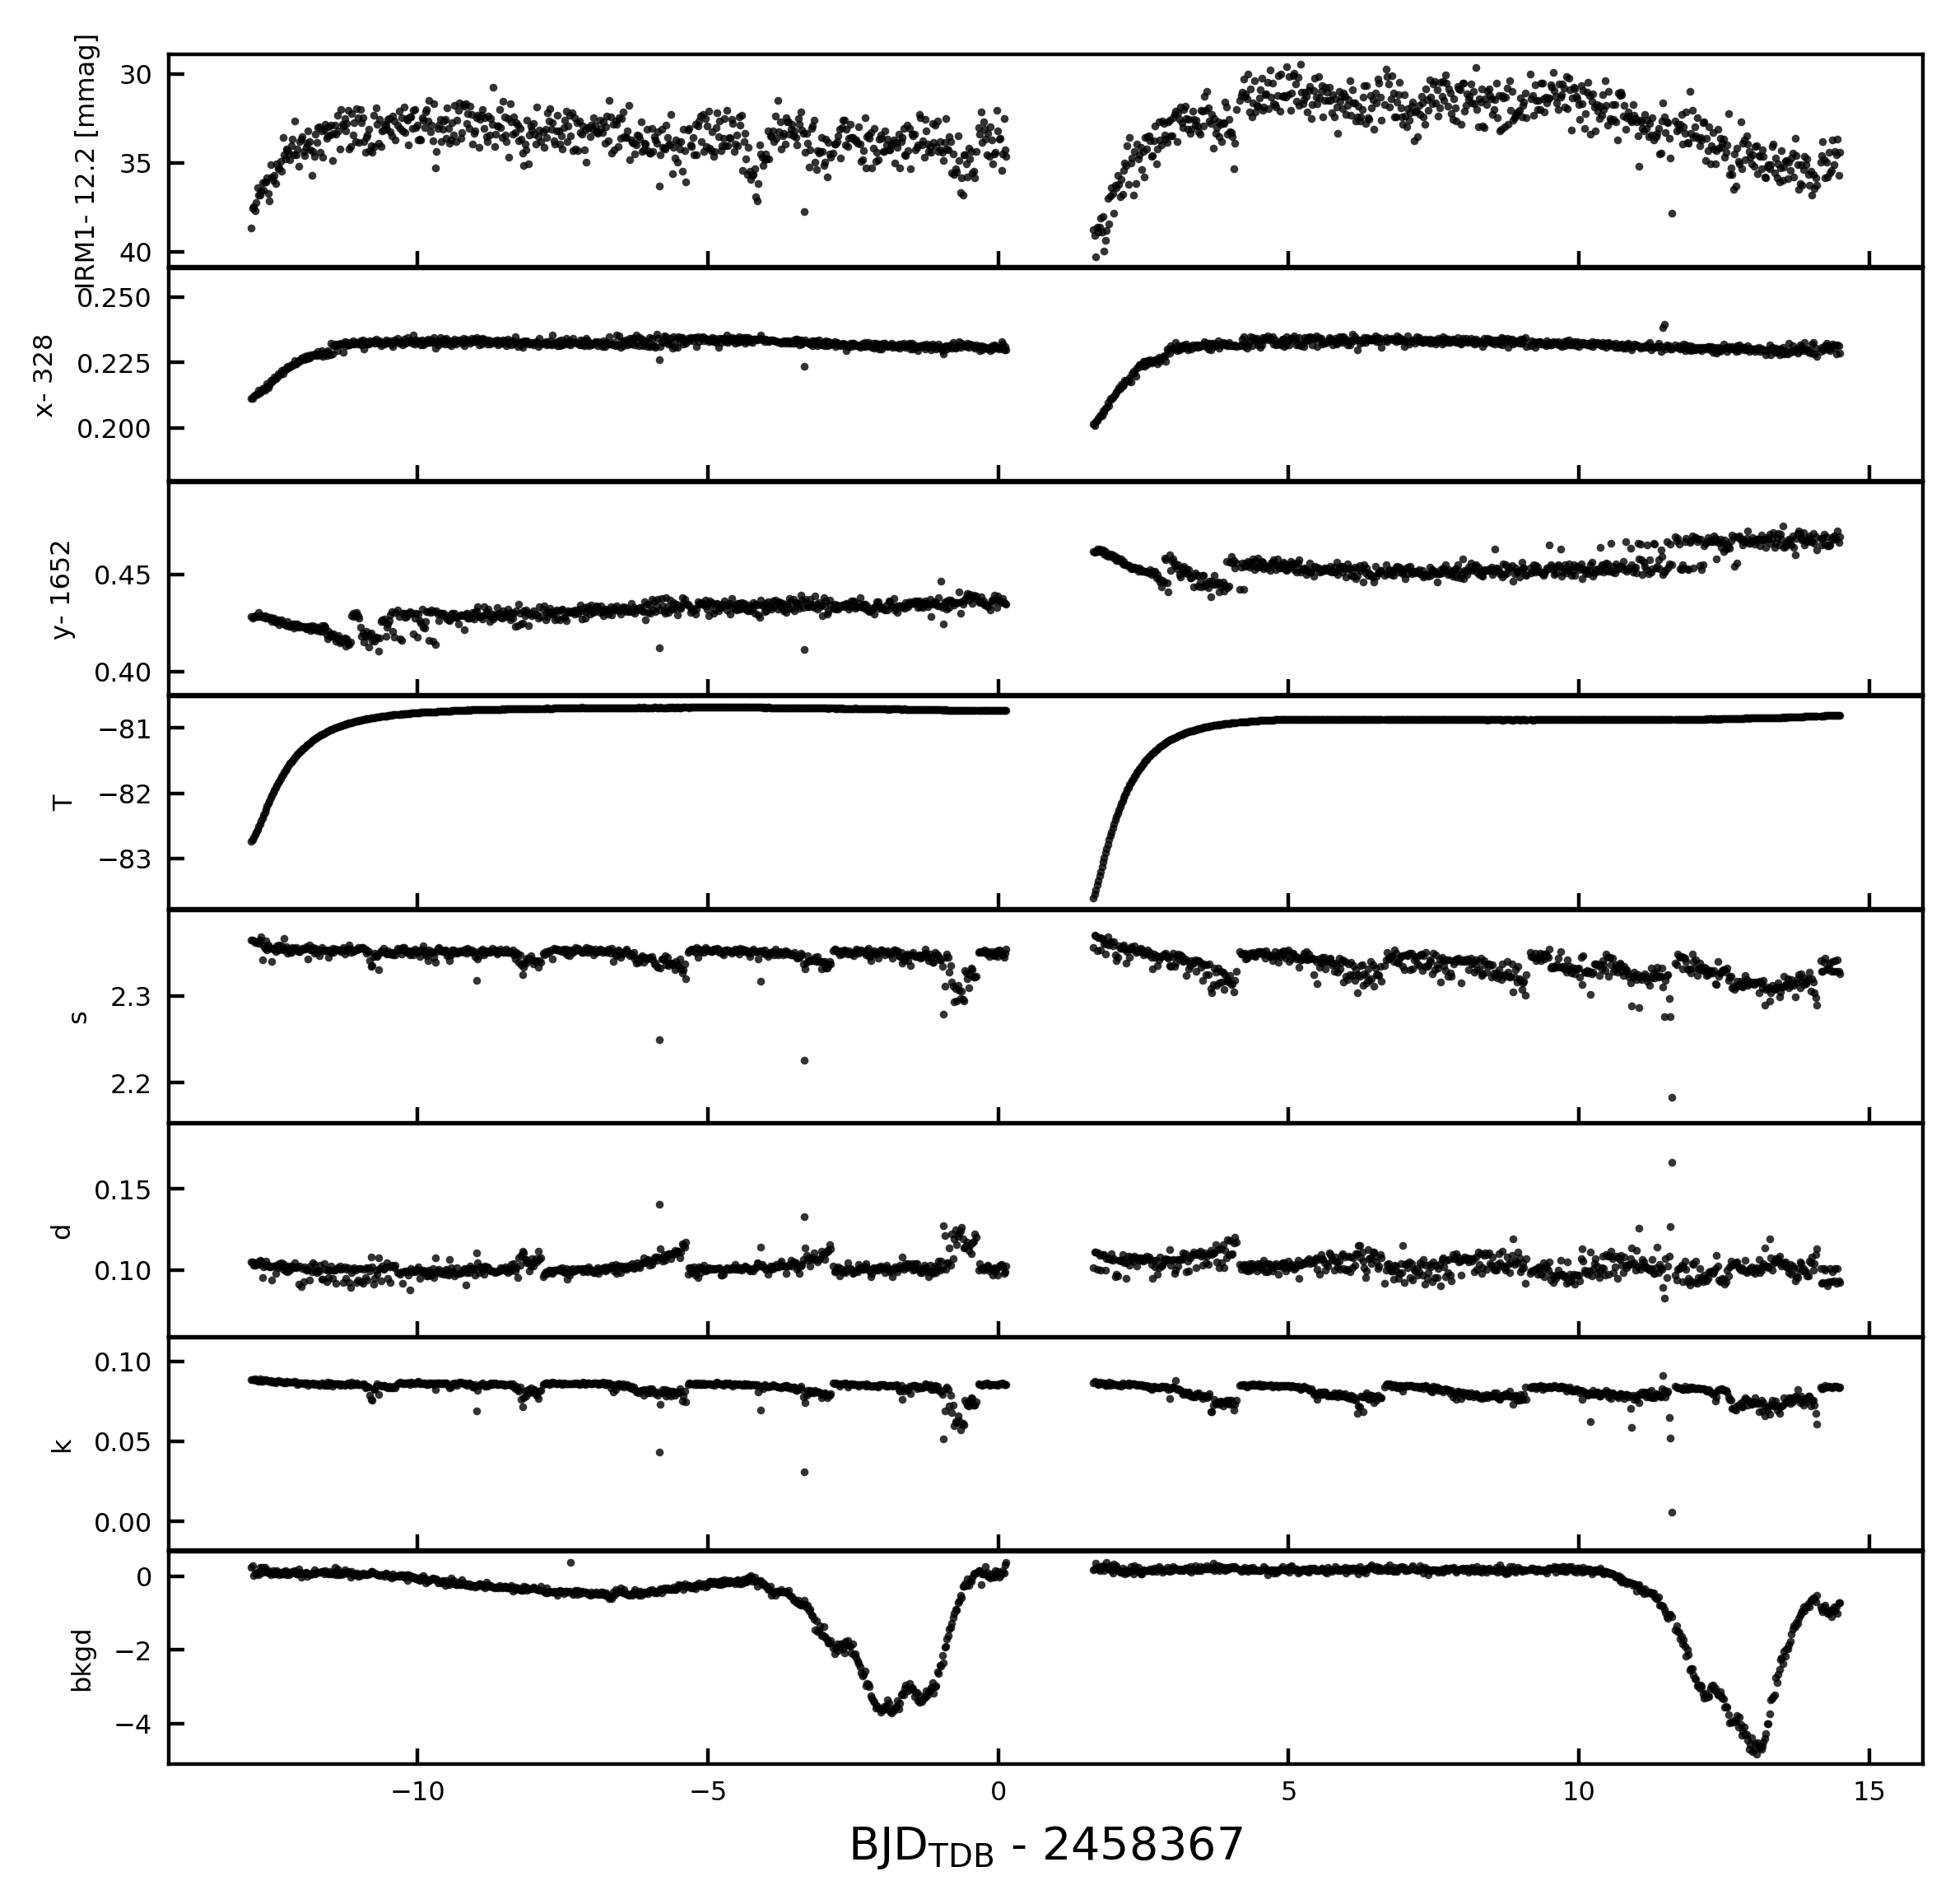
\includegraphics[width=0.6\textwidth]{epdparams_vs_time.png}
	\end{center}
	\vspace{-0.5cm}
	\caption{
    {\bf Timeseries of ``external parameters'' for a representative
    star.} {\it Top}: Instrumental raw magnitude (with a particular
    aperture size), as a function of time.  {\it Second and third from
    top}: $x$ and $y$ centroid positions as a function of time.
    Continuing in order are the CCD temperature, the $(s,d,k)$ shape
    parameters, and the measured background value.
    Most of the apparent variability is instrumental: see
    \S~\ref{sec:flux_vs_external_parameters}.
		\label{fig:external_parameter_timeseries}
	}
\end{figure*}


\begin{figure*}[t]
    \begin{center}
		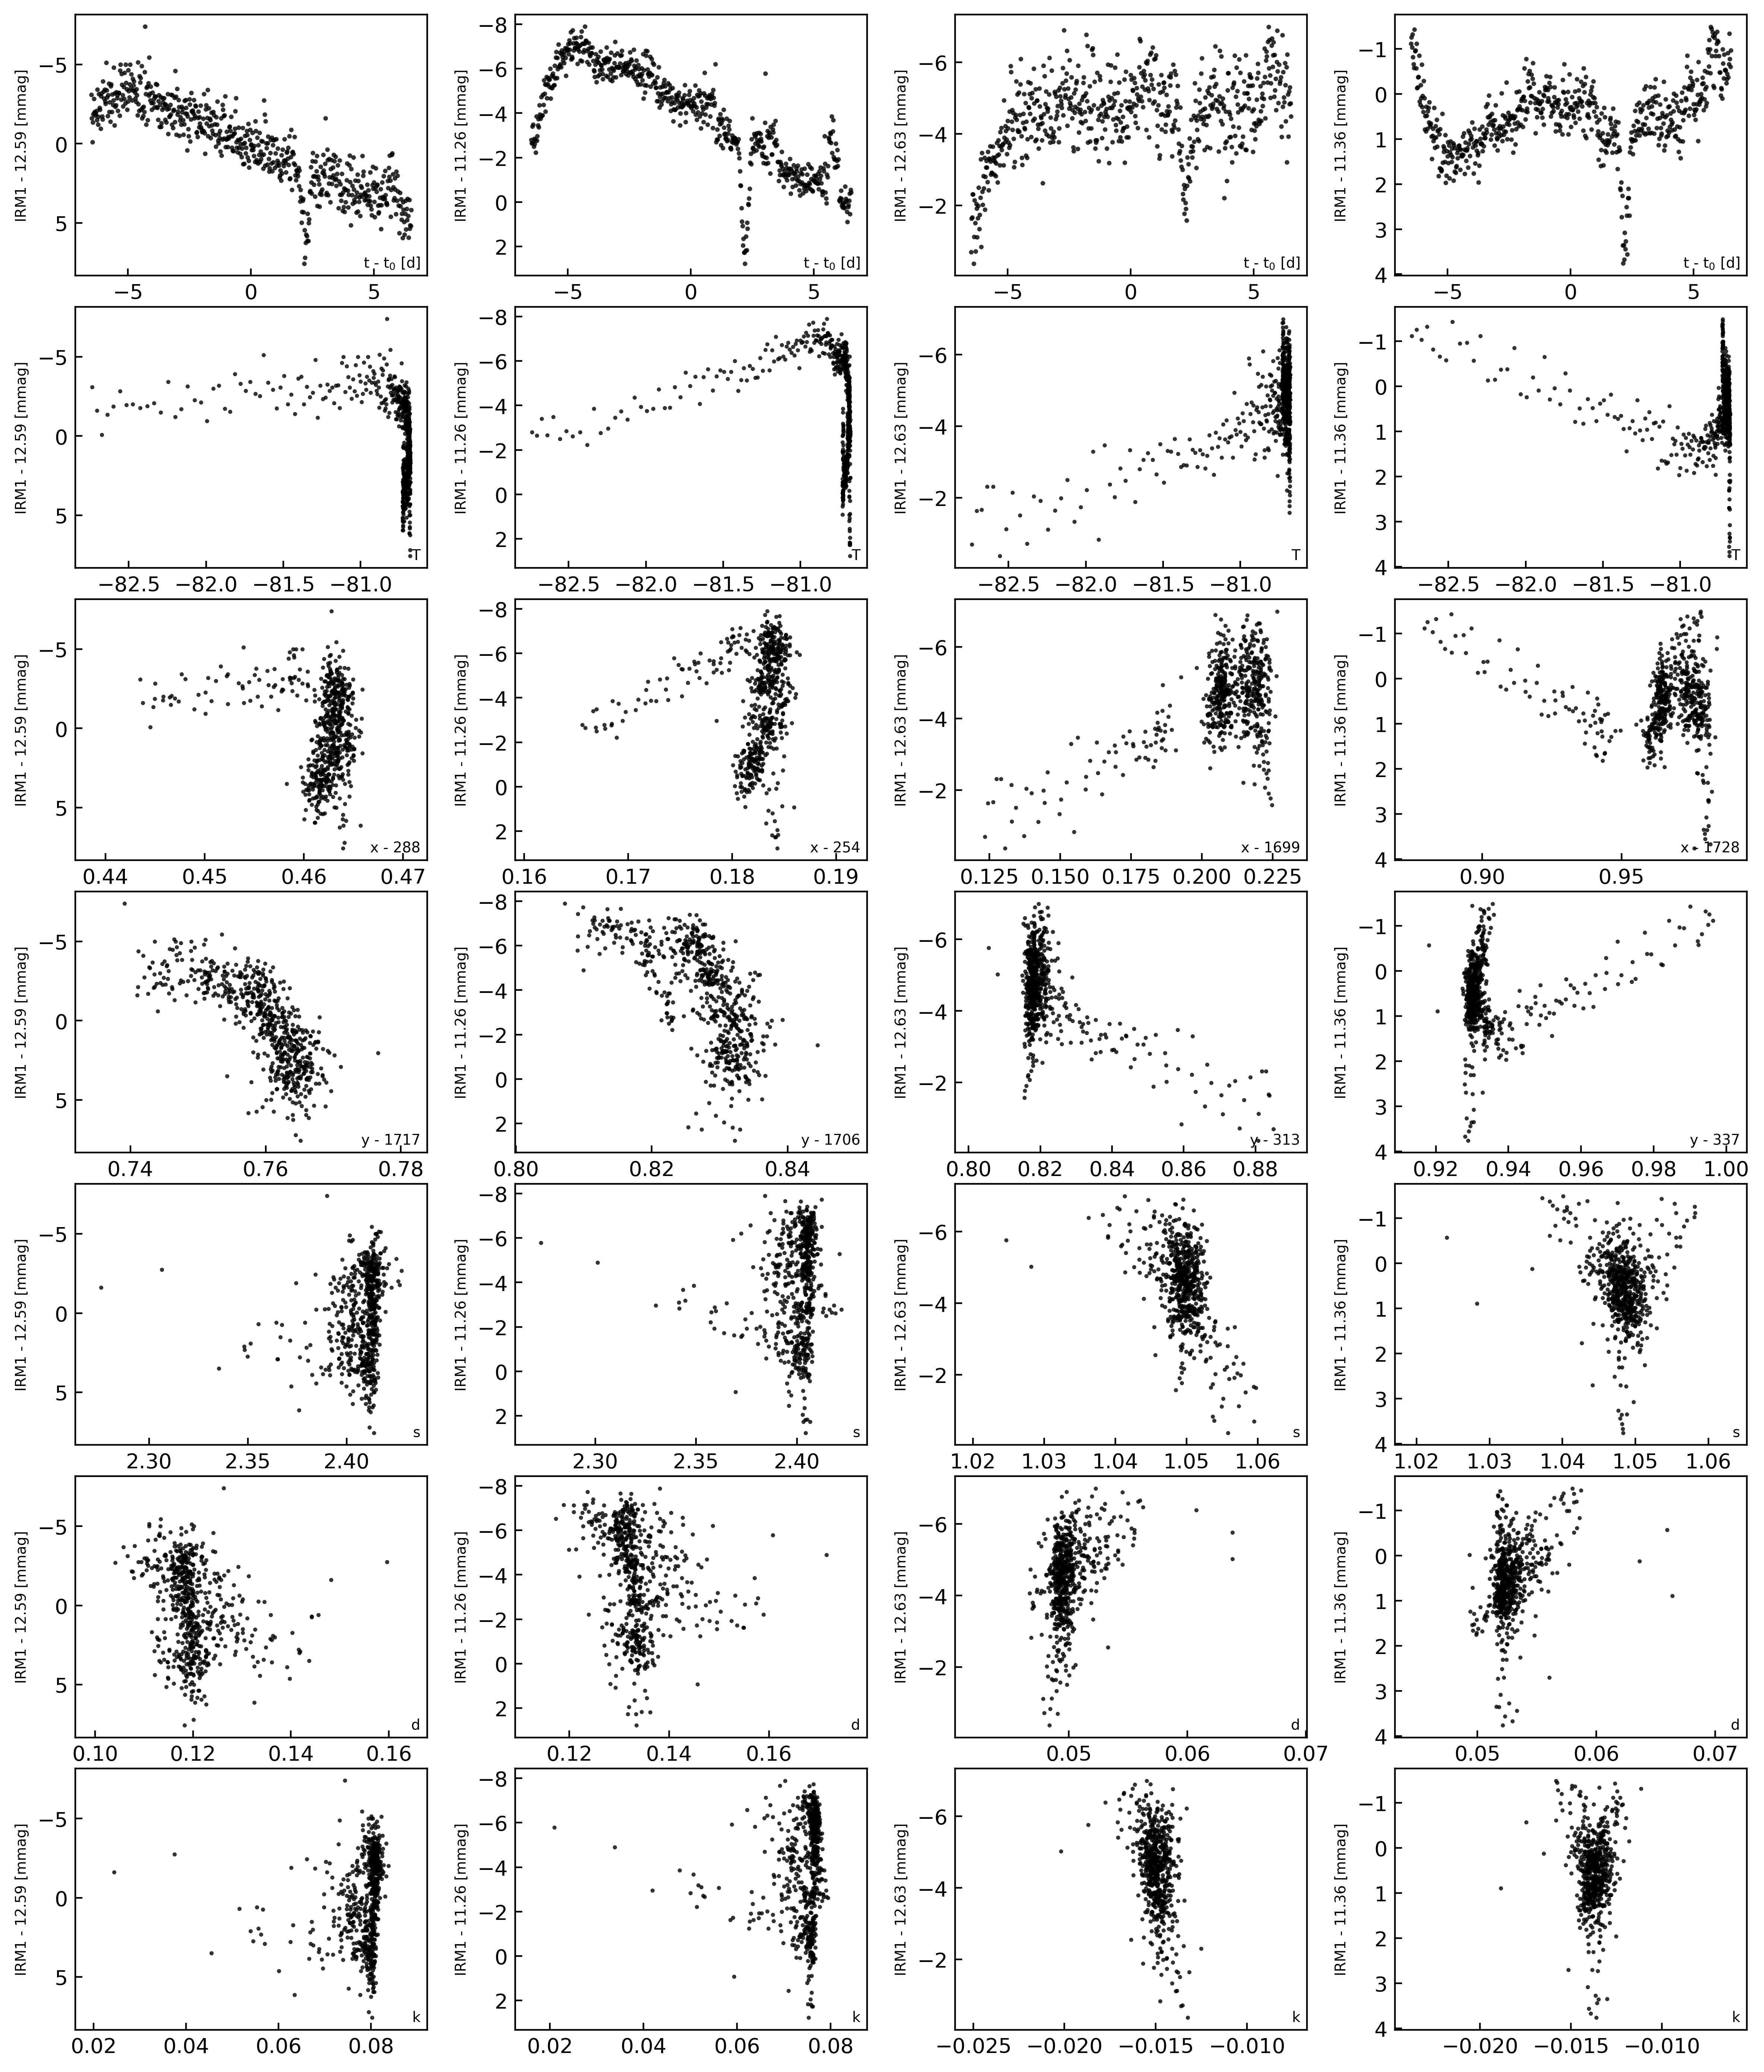
\includegraphics[height=0.9\textheight]{mag_vs_epdparams.png}
    \end{center}
    \vspace{-0.5cm}
    \caption{
      {\bf Flux as a function of ``external parameters'' for four
      representative stars.} The left two columns are stars at the
      corner of a camera's field; the right two columns are from the
      centers.
      Each row shows a different parameter along the $x$-axis, given
      in text at the bottom right of each subplot.
      ``Hooks'' are common features in flux as a function of
      temperature and centroid position.
      \S~\ref{sec:flux_vs_external_parameters} gives a verbose
      description.
     \label{fig:flux_vs_external_parameters}
    }
\end{figure*}

The traditional approach to EPD is to fit and
subtract a model for the magnitudes $m$ of the form
\begin{equation}
  m = {\rm const.} + \sum_i c_i \theta_i,
  \label{eq:classical_EPD}
\end{equation}
where $\vec{\theta}$ is a vector of parameters such as the shape
parameters $(s,d,k)$, their products $(s^2, s\cdot d, d^2, \ldots)$,
the temperature $T$ of the instrument or environment\footnote{ We used
the temperature from the on-chip aluminum-copper sensor measurements
included in the engineering
data: \url{archive.stsci.edu/missions/tess/engineering/}.  },
the centroid positions $(x,y)$, the fractional part of the
centroid positions $(\{x\},\{y\})$, and any other parameters that are
expected\footnote{ The fractional centroid positions might matter
because intra-pixel quantum efficiency variations could affect the
measured stellar brightness.  The varying temperature $T$ of the CCD
electronics might matter.  } to correlate strongly with the observed
flux.  The coefficients $c_i$ are calculated through linear
least-squares, and subtracted to produce ``EPD'' light curves.

The premise of this model is that the correlations between the
magnitudes and the external parameters are linear.  For ground-based
CCD data (e.g., HATNet, HATS, and Nikon DSLRs), \citet{bakos_2010} and
\citet{zhang_precision_2016} have verified that this model is a
good description to the data.
To discern whether such a model extends to the TESS data, we examined
scatter plots of each parameter, as a function of all the other
parameters.  We also examined plots of each parameter as a function of
time.  A few prominent trends were present.

\begin{enumerate}

\item {\it Flux vs.\ time}. Most of the light curves we examined showed a secular
    drift with amplitude $0.01\,{\rm mag}$ over the timescale of each
    orbit.  Sharper trends (``hooks'') at the beginning of each orbit
    seemed to be less prominent for stars at the corners of the fields
    than stars at the center.  The periodicity incurred by the
    2.5$\,{\rm day}$ momentum dumps was also noticeable in more of the
    light curves at the center of the field than at the corners.

\item {\it Flux vs.\ centroid positions}. The flux as a function of
  centroid position often showed non-linear ``hooks'' (see Figure
    \ref{fig:flux_vs_external_parameters}). Most of the data points from a 
    given orbit reside at a given
    level, but about 10\% are in a tail. This was seen in light curves
    all across the TESS field of view.

\item {\it Flux vs.\ temperature} exhibited similar hooks, with most of
  the flux values residing at a particular level, and perhaps 10\%
    following a non-linear path (often resembling the Nike ``swoosh'')
    away from the bulk of points.

\item {\it Flux vs.\ shape parameters}.  For light curves in the corner
  of the field of view, similar hooks are present in flux {\it vs.}
    $(s,d,k)$, though the hooks are less sharp.  In the center of the
    field of view, gaussian ellipses are a better description of the
    flux {\it vs.} the shape parameters.
    
\end{enumerate}

Considering the timeseries of parameters other than flux 
(Figure~\ref{fig:external_parameter_timeseries}):

\begin{enumerate}

\item {\it Centroid positions vs\ time}.  The main variability in the
  centroid positions as a function of time is a secular drift, that is
    reset every orbit.  The 2.5 day momentum wheel dump is
    superimposed on this secular drift, and has smaller amplitude than
    the drift.

\item {\it Temperature vs.\ time}.  The main variability in temperature
  {\it vs.} time is a secular drift of the same timescale as that for
    the centroid positions timeseries.

\item {\it Shape parameters vs.\ time}.  The main variability in the
  shape parameters as a function of time is the 2.5 day momentum wheel
    dump periodicity, with hooks before each momentum dump.

\item {\it Background value vs.\ time}.  The background is typically stable, 
except when scattered light from the Earth or Moon enters the frame (visible 
towards the end of each orbit in 
Figure~\ref{fig:external_parameter_timeseries}).

\end{enumerate}

Given the characteristics of the variability, a linear model of the
form given in Equation~\ref{eq:classical_EPD} is not applicable.  To
fit out the correlations between flux and parameters which most
commonly exhibited ``hooks'', we explored fitting a parametric open
curve (an $N$-dimensional B-spline, \citealt{dierckx_curve_1996}) to
the flux, centroid positions, and temperatures simultaneously.  We
selected the number of knots through brute-force, by calculating
$\chi^2$ for the model fit over a grid of possible knots, and
minimizing the Bayesian Information Criterion.  Though this approach
showed some initial promise, even with ``optimal'' knot-selection (in
the BIC sense) it introduced undesirable residuals in the light curves,
and also distorted transits.
One thought that we did not try but may explore in future work
is to use the decorrelate against the scatter of the quartnerion 
time-series (CITE: Vanderburg, 2019).

Given these complications, for the time being we omit the step of
``detrending'' as a function of external parameters. To
enable further exploration of the issue, we include all the necessary
vectors of {\it e.g.}, centroid positions, temperatures, and shape
parameters in our reported light curves.
	


\subsubsection{Trend filtering algorithm}
\label{sec:tfa_is_good_enough}


Since most of the external parameter dependence is shared between
stars, we opt to decorrelate the flux timeseries of each star
against other stars in the frame.
We use the TFA algorithm proposed by
\citet{kovacs_trend_2005}, which for self-consistency we reproduce
here.
The idea of the method is somewhat simpler than the PDCMAP
algorithm used in the SPOC pipeline (CITE).
Suppose we have $M$ ``template stars'', which are a subsample of
stars that represent all types of systematics across the dataset. 
Each template star has a light curve with $N$ data points.
Denote the template time-series $X_j(i)$, where $j={1,\ldots,M}$ and 
$i={1,\ldots,N}$ is the time index.
We then want to find periodic signals in a target time-series $Y(i)$.
This is done by defining a filter function
\begin{equation}
F(i) = \sum_{j=1}^{M} c_j X_j(i),
\end{equation}
for which the coefficients $c_j$ are found by minimizing
\begin{equation}
\mathcal{D} = \sum_{i=1}^{N} \left[ Y(i) - A(i) - F(i) \right]^2.
\label{eq:tfa_to_minimize}
\end{equation}
When trying to find periodic signals, $A(i)$ represents our prior
knowledge of the light curve's shape.
This prior is simply that stars on average maintain a constant brightness:
\begin{equation}
A(i) = \langle Y \rangle = \frac{1}{N} \sum_{i=1}^{N} Y(i) = {\rm const.}
\end{equation}
If a signal is eventually found, for instance using the box-least squares
method \citep{kovacs_box-fitting_2002},
this detrending process must then be repeated while accounting for our
updated knowledge about the light curve's shape.

Some notes on our implementation follow.
We select template stars in two stages.
In the first stage, we fit a parabola in the RMS-magnitude
plane, and discard stars more than $2\sigma$ away from the
prediction of the fit.
We also require that these initial candidate stars have intermediate
brightness ($8.5 > T > 13$), and have a relatively large number
of time-series data points.
We then perform an initial iteration of TFA, on only the candidate
template stars.
We inspect the resulting detrended light curves for residual
structure by computing a Lomb-Scargle periodogram.
If the maximum-power peak has a false alarm probability below 0.1\%, 
we exclude the star from the list of candidate template stars, on the
basis of its presumed periodic variability.
We then randomly select at most 200 template stars from the remaining
non-variable candidates. 
The choice of number of template stars was discussed by
\citet{Kovacs_et_al_2005}, and is another free parameter in
the broad problem of light curve production.
While it can be optimized by constructing and minimizing a BIC-like 
quantity, a little overfitting is acceptable for our puposes.

Once the template stars are selected, we use the \texttt{VARTOOLS}
program to perform the detrending \citep{Hartman_Bakos_2016}.
This process is performed for each photometric aperture
separately.


%%%%%%%%%%%%%%%%%%%%%%%%%%%%%%%%%%%%%%%%%%
\section{Results}
\label{sec:results}

\subsection{Light Curve Statistics}

\begin{figure}[t]
	\begin{center}
		\leavevmode
		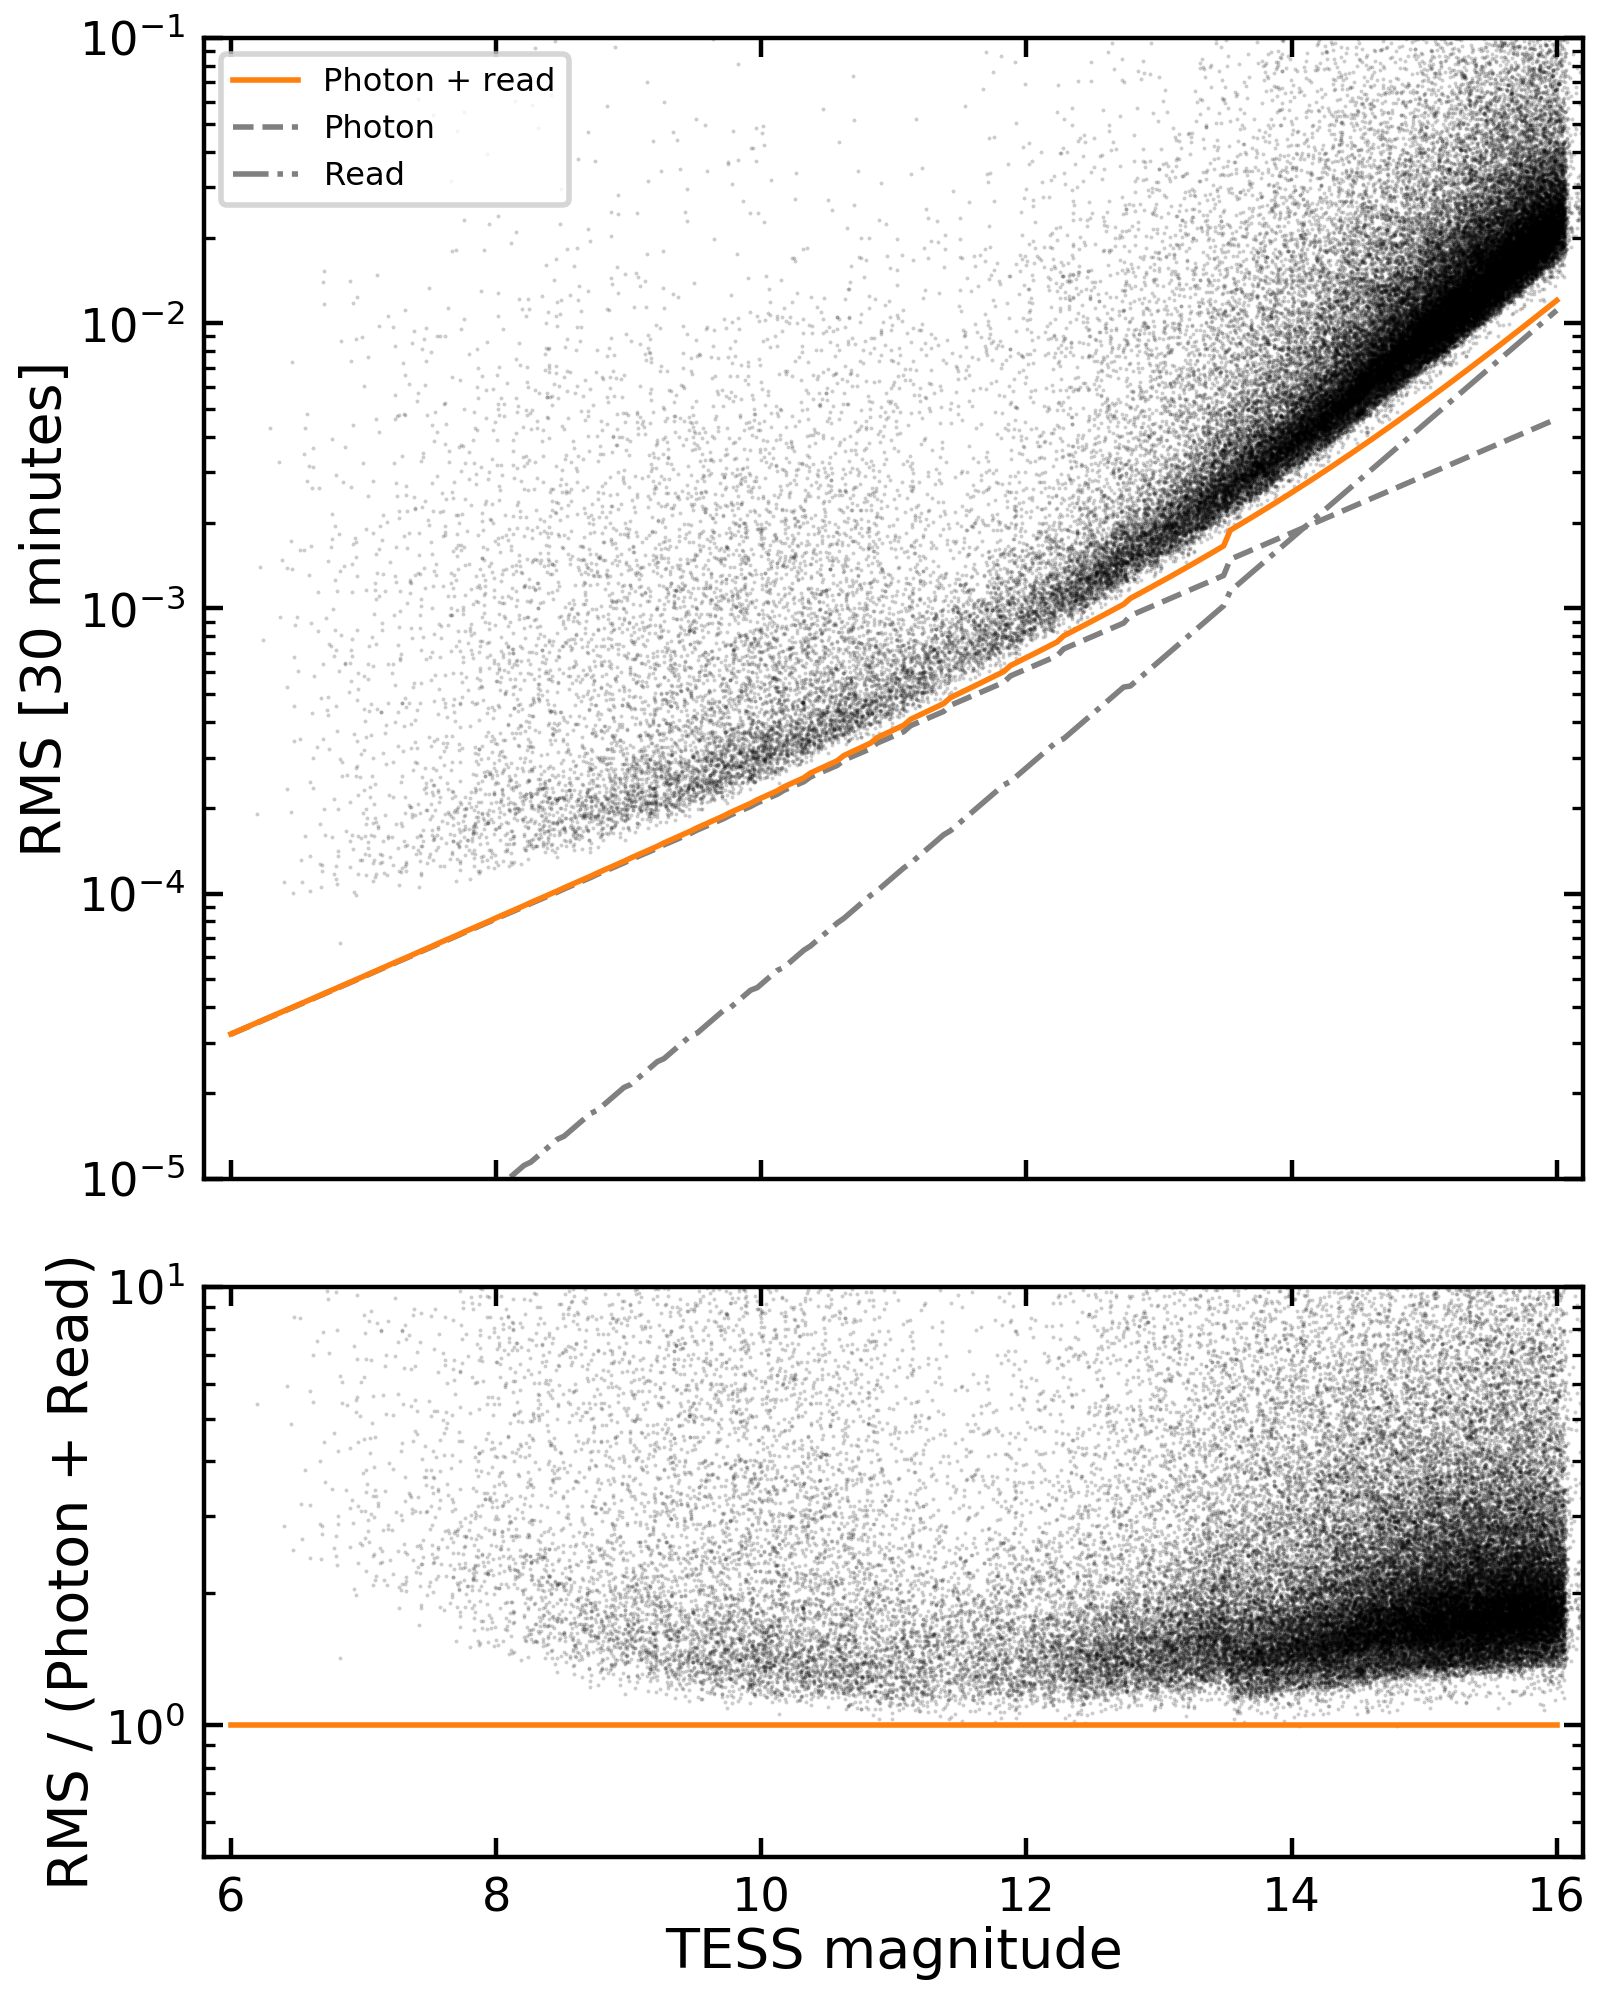
\includegraphics[width=0.49\textwidth]{rms_vs_mag.png}
	\end{center}
	\vspace{-0.5cm}
  \caption{ {\bf Standard deviation of light curves vs catalog
  TESS-band magnitude for CDIPS light curves.}  Faint stars in heavily
  crowded regions have bright neighbors which drive their light curve
  scatter below the expected noise limits.
		\label{fig:rms_vs_mag}
	}
\end{figure}

\begin{figure}[t]
	\begin{center}
		\leavevmode
		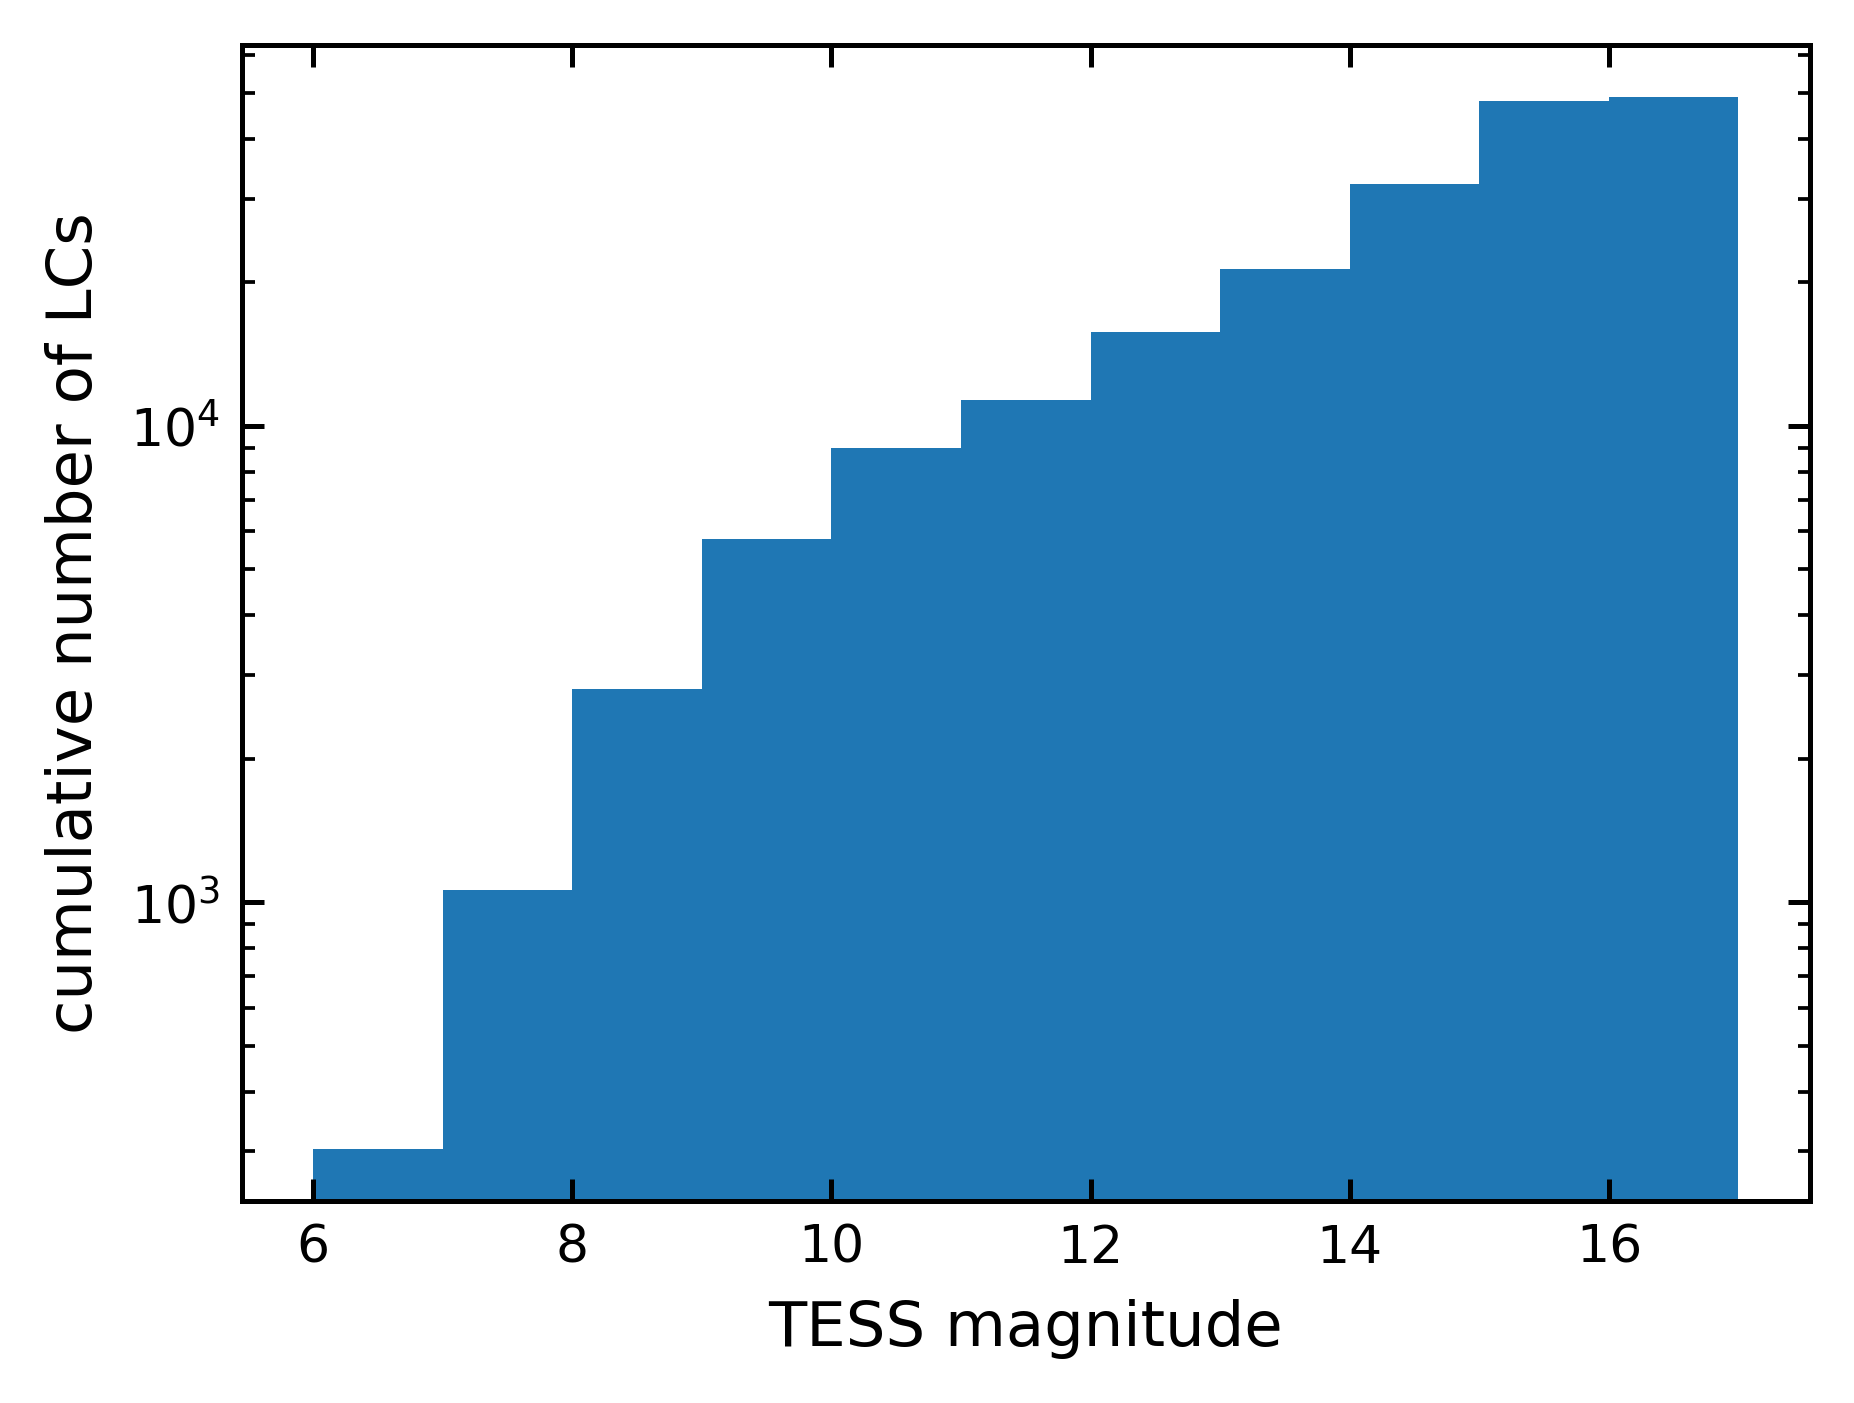
\includegraphics[width=0.45\textwidth]{cdf_T_mag.png}
	\end{center}
	\vspace{-0.5cm}
	\caption{
		{\bf Cumulative distribution of TESS-band magnitudes for CDIPS light curves.}
		\label{fig:cdf_T_mag}
	}
\end{figure}

\begin{figure}[!ht]
	\gridline{\fig{hrd_scat_all_CDIPS_LCs.png}{0.45\textwidth}{}}
	\vspace{-0.8cm}
	\gridline{\fig{hrd_scat_close_subset.png}{0.45\textwidth}{}}
	\caption{
		{\it Top.} Stellar properties of CDIPS stars with light curves in this data release.
		{\it Bottom.} Stellar properties of close CDIPS stars with light curves.
	}
	\label{fig:hrd}
\end{figure}


ACF statistics before and after detrending(?)

SNR of retrieved HJs.

Maybe movies of subtracted images?

Some stellar variability plots (perhaps of known stellar variables).

Some focus on particular clusters.

\subsection{Objects of Interest}
\label{subsec:ctois}

As an initial search for transiting planets, strong stellar rotators, and 
eclipsing binaries, we performed a few steps of post-processing. For 
simplicity,
we chose a single aperture size~--~``aperture 2''~--~with a radius of 1.5 
pixels, to perform the period search.

First, to identify periodic transit-like signals, we used 
\citet{hippke_TLS_2019}'s transit least-squares (TLS) tool.
The algorithm is the same as the canonical box least-squares
\citep{kovacs_box-fitting_2002}, except in place of a box template, a transit 
template is used  for a marginal improvement of the detection efficiency.
In addition, the search grids in \texttt{tls} 
\footnote{\url{https://github.com/hippke/tls}} are slightly more 
efficient than in most BLS implementations, since \texttt{tls} uses the 
cubic-in-frequency sampling advocated by \citet{ofir_optimizing_2014}, 
rather than standard linear-in-frequency sampling.
During the period search, we rejected $6\,{\rm hours}$ at the
beginning and end of each spacecraft orbit, to mitigate the presence
of correlated red noise in the results.
This shrinks the data volume by about 5\%, but also lowers the number
of systematic false positives in subsequent vetting.
Our grids typically consisted of about 25 different durations, and
about 2500 periods between 0.5 and 11 days.
We also ran a generalized Lomb-Scargle periodogram (CITE), simply to 
have additional periodicity information.

We then performed a cut on the TLS signal detection efficiency:
${\rm SDE} > 12$.
This yielded XXX light curves, and we then
performed TFA signal reconstruction on these lightcurves using 
\texttt{vartools}.
In this process, the model lightcurve $A(i)$ in 
Equation~\ref{eq:tfa_to_minimize} is set to the phase-binned signal from the 
most powerful peak in the TLS spectrum, rather than being a constant function. 
Generally speaking, this helps improve the quality of the resulting light 
curve.

We then make a multi-page \texttt{.pdf} document with the information 
necessary to make classifications for vetting.
These documents are released along with the light curves, as a useful summary
 for anyone interested in the subset of objects that we have analyzed.
A full description of each page of the summary \texttt{.pdf} is given in the 
Appendix.

The classifications we used assess:
\begin{enumerate}
    \item {\it The source of photometric variability}. Designations include 
    tags for planet candidates, eclipsing binaries, instrumental variations, 
    stellar variations, and ``weirdos''.
    \item {\it Cluster membership status}. By default, all light curves were 
    made for stars with at least one literature claim of cluster membership.  
    We therefore include tags only for non-cluster members, and possible 
    non-cluster members. Typically the primary source of this information is 
    the Gaia-DR2 parallax.
    \item {\it Photometric blends}. Tags are created to highlight whether the 
    depth of the photometric signal shows a strong dependence on aperture 
    size, and also whether the in-transit minus the out-of-transit images 
    reveal that the source of variability is in fact far from the target star.
\end{enumerate}
The actual classification process was performed by LGB, JH, and JNW.
The \texttt{TagSpaces} software was used~--~an extremely helpful tool for the 
purposes of easily assigning labels to documents.



% FIXME FIXME FIXME



%%%%%%%%%%%%%%%%%%%%%%%%%%%%%%%%%%%%%%%%%%
\section{Discussion}
\label{sec:discussion}

Lorem ipsum.

%%%%%%%%%%%%%%%%%%%%%%%%%%%%%%%%%%%%%%%%%%
\section{Conclusion}
\label{sec:conclusion}

% \begin{figure}[t]
% 	\begin{center}
% 		\leavevmode
% 		\includegraphics[width=0.49\textwidth]{f6.pdf}
% 	\end{center}
% 	\vspace{-0.5cm}
% 	\caption{
%     {\bf Further observations will be needed to confirm and understand
%     the timing variations of WASP-4b.} Dots are as in
%     Figure~\ref{fig:times}.  Lines are 100 random draws from the
%     posteriors of the apsidal precession model (orange), and the
%     orbital decay model (blue).    
% 		\label{fig:future}
% 	}
% \end{figure}




\acknowledgements
L.G.B.\ gladly acknowledges helpful discussions with
..., and is
grateful to the people who have turned TESS from an idea into reality.
%
J.N.W.\ thanks ...
%
This paper includes data collected by the TESS mission, which are
publicly available from the Mikulski Archive for Space Telescopes
(MAST).
%
Funding for the TESS mission is provided by NASA's Science Mission
directorate.
%
This research has made use of the NASA Exoplanet Archive, which is
operated by the California Institute of Technology, under contract
with the National Aeronautics and Space Administration under the
Exoplanet Exploration Program.
%
This work made use of NASA's Astrophysics Data System Bibliographic
Services.
%
This research has made use of the VizieR catalogue access tool, CDS,
Strasbourg, France. The original description of the VizieR service was
published in A\&AS 143, 23.
%
This work has made use of data from the European Space Agency (ESA)
mission {\it Gaia} (\url{https://www.cosmos.esa.int/gaia}), processed
by the {\it Gaia} Data Processing and Analysis Consortium (DPAC,
\url{https://www.cosmos.esa.int/web/gaia/dpac/consortium}). Funding
for the DPAC has been provided by national institutions, in particular
the institutions participating in the {\it Gaia} Multilateral
Agreement.
%
\newline
%
\facility{
	TESS \citep{ricker_transiting_2015},
	Gaia \citep{gaia_collaboration_gaia_2016,gaia_collaboration_gaia_2018},
	2MASS \citep{skrutskie_tmass_2006},
    DSS (CITE)    
}
%
\software{
  \texttt{astrobase} \citep{bhatti_astrobase_2018},
  \texttt{astropy} \citep{the_astropy_collaboration_astropy_2018},
  \texttt{astroquery} \citep{astroquery_2018},
  \texttt{astroquery.gaia}
  \texttt{astroquery.simbad}
  \texttt{astroquery.mast}
  \texttt{astroquery.nasaexopanetarchive}  
  \texttt{BATMAN} \citep{kreidberg_batman_2015},
  \texttt{corner} \citep{corner_2016},
  \texttt{emcee} \citep{foreman-mackey_emcee_2013},
  \texttt{fitsh} \citep{Pal_2012},
  \texttt{IPython} \citep{perez_2007},
  \texttt{matplotlib} \citep{hunter_matplotlib_2007}, 
  \texttt{numpy} \citep{walt_numpy_2011}, 
  \texttt{pandas} \citep{mckinney-proc-scipy-2010},
  \texttt{scipy} \citep{jones_scipy_2001},
  \texttt{TagSpaces} (CITE),
  \texttt{tesscut} (CITE)
}

\bibliographystyle{yahapj}                            
\bibliography{bibliography} 

\appendix
\section{Time system \& barycentric correction}
The time-stamps included with the calibrated TESS Full Frame Images
produced by SPOC include a barycenteric correction at
a single reference pixel given at the middle of every frame.
The barycentric correction is at maximum 16 minutes, corresponding to
points on the sky separated by 180 degrees.
The angular distance from a TESS camera's center of field to the corners
is $\approx$17 degrees, so naively one might incur at worst an error of
$\approx$90 seconds on the time-stamps due to using a barycentric
correction in a direction that is slightly wrong.
Perhaps due to the lead author's obsession with getting time-stamps correct 
\citep{bouma_wasp-4b_2019},
we perform our own barycentric correction using the appropriate
sky coordinates for each light curve.
We advise use of our \texttt{TMID\_BJD} column, which gives the
mid-time of each exposure in the BJD$_{\rm TDB}$ time system, which
is the defacto standard in exoplanet and stellar
astronomy~\citep{eastman_achieving_2010}.

\section{Vetting Document Description}

In \S~\ref{subsec:ctois}, we described the process by which we made 
\texttt{.pdf} documents suitable for assessing which objects were interesting 
enough to merit further study.

This section briefly summarizes this document. Updated versions and their 
\texttt{README} files will live at this web-address: 
\url{mast.stsci.edu/CDIPS}.

\begin{itemize}
\item {\it Page 1: period-search summary}. Periodograms from TLS and 
phase-dispersion minimization 
\citep{hippke_TLS_2019,stellingwerf_period_1978}, as calculated 
with \texttt{astrobase.periodbase} are shown. The top three peaks from each 
method are shown in the second and third rows; the raw light curve is in the 
top-right. A small finder chart from DSS is shown (CITE).

\item {\it Page 2: light curve diagnostics}.
\end{itemize}


\end{document}

